% 五列四子棋在任意有限高度上都是和棋
% 单文件源码。编译：xelatex five_columns_draw_zh.tex（在干净目录中运行三次）。
% 需要 TeX Live 与字体 Noto Serif CJK SC、Noto Sans CJK SC、Noto Sans Mono CJK SC、Linux Libertine O。
% ===== preamble.tex =====
\documentclass[11pt,a4paper]{article}

\usepackage[a4paper,margin=22mm]{geometry}
\usepackage{amsmath,amssymb}
\usepackage[sc]{mathpazo}
\usepackage{fontspec}
\usepackage{babel}
\babelprovide[import,main]{chinese}
% Chinese has no italic: emphasis (defined terms, run-in heads) is set in the sans face, as is customary
\babelfont{rm}[Ligatures=TeX,ItalicFont={Noto Sans CJK SC},BoldItalicFont={Noto Sans CJK SC Bold}]{Noto Serif CJK SC}
\babelfont{sf}{Noto Sans CJK SC}
\babelfont{tt}[Scale=0.92]{Noto Sans Mono CJK SC}
\newfontfamily\latinrm{Linux Libertine O}[Ligatures=TeX]
% Line breaks between Chinese text and inline math, code or references
\XeTeXinterchartokenstate=1
\chardef\zhIdeo=1 \chardef\zhClose=2 \chardef\zhOpen=3
\count255="3400 \loop\XeTeXcharclass\count255=\zhIdeo \ifnum\count255<"4DBF \advance\count255 by 1 \repeat
\count255="4E00 \loop\XeTeXcharclass\count255=\zhIdeo \ifnum\count255<"9FFF \advance\count255 by 1 \repeat
\XeTeXcharclass`，=\zhClose \XeTeXcharclass`。=\zhClose \XeTeXcharclass`；=\zhClose
\XeTeXcharclass`：=\zhClose \XeTeXcharclass`、=\zhClose \XeTeXcharclass`！=\zhClose
\XeTeXcharclass`？=\zhClose \XeTeXcharclass`）=\zhClose \XeTeXcharclass`”=\zhClose
\XeTeXcharclass`’=\zhClose \XeTeXcharclass`》=\zhClose \XeTeXcharclass`】=\zhClose
\XeTeXcharclass`（=\zhOpen \XeTeXcharclass`“=\zhOpen \XeTeXcharclass`‘=\zhOpen
\XeTeXcharclass`《=\zhOpen \XeTeXcharclass`【=\zhOpen
% A break point is added only where the previous node is not glue or a penalty, so that
% ties (~) and spaces keep their meaning; none is kept before a closing mark or after an opening one.
\newif\ifzhafteropen
\def\zhbreak{\ifnum\lastnodetype>-1 \ifnum\lastnodetype<11 \allowbreak\fi\fi}
\XeTeXinterchartoks\zhIdeo 4095={\zhbreak}
\XeTeXinterchartoks\zhClose 4095={\zhbreak}
\XeTeXinterchartoks\zhOpen 4095={\global\zhafteropentrue}
\XeTeXinterchartoks 4095 \zhIdeo={\ifzhafteropen\global\zhafteropenfalse\else\zhbreak\fi}
\XeTeXinterchartoks 4095 \zhOpen={\global\zhafteropenfalse\zhbreak}
\XeTeXinterchartoks 4095 \zhClose={\global\zhafteropenfalse\unpenalty}
% babel makes ~ a shorthand; let it also remove a break point inserted just before it
\makeatletter\declare@shorthand{system}{~}{\leavevmode\unpenalty\nobreak\ }\makeatother






\usepackage{amsmath,amssymb,amsthm,mathtools}
\usepackage{xcolor}
\usepackage{booktabs,tabularx,array}
\usepackage[font=small,labelfont=bf]{caption}
\usepackage{enumitem}
\usepackage{tikz}
\usetikzlibrary{arrows.meta,positioning,calc,decorations.pathreplacing}
\PassOptionsToPackage{obeyspaces,spaces}{url}
\usepackage{hyperref}
\usepackage[nameinlink]{cleveref}
\crefname{section}{第}{第}\creflabelformat{section}{#2#1#3~节}
\Crefname{section}{第}{第}
\crefname{subsection}{第}{第}\creflabelformat{subsection}{#2#1#3~节}
\Crefname{subsection}{第}{第}
\crefname{appendix}{附录}{附录}\Crefname{appendix}{附录}{附录}
\crefname{theorem}{定理}{定理}\Crefname{theorem}{定理}{定理}
\crefname{lemma}{引理}{引理}\Crefname{lemma}{引理}{引理}
\crefname{corollary}{推论}{推论}\Crefname{corollary}{推论}{推论}
\crefname{proposition}{命题}{命题}\Crefname{proposition}{命题}{命题}
\crefname{definition}{定义}{定义}\Crefname{definition}{定义}{定义}
\crefname{example}{例}{例}\Crefname{example}{例}{例}
\crefname{remark}{注}{注}\Crefname{remark}{注}{注}
\crefname{table}{表}{表}\Crefname{table}{表}{表}
\crefname{figure}{图}{图}\Crefname{figure}{图}{图}
\crefname{enumi}{}{}
\newcommand{\crefpairconjunction}{与}
\newcommand{\crefmiddleconjunction}{、}
\newcommand{\creflastconjunction}{与}
\newcommand{\crefrangeconjunction}{至}

\definecolor{primary}{RGB}{20,54,93}
\definecolor{accent}{RGB}{18,110,98}
\definecolor{warn}{RGB}{168,50,50}
\definecolor{gold}{RGB}{176,120,20}
\definecolor{softbg}{RGB}{244,247,251}
\definecolor{gridgray}{RGB}{176,184,194}
\definecolor{stoneB}{RGB}{30,30,30}

\hypersetup{
  colorlinks=true,
  linkcolor=primary,
  citecolor=accent,
  urlcolor=primary,
  pdftitle={五列四子棋在任意有限高度上都是和棋},
  pdfauthor={GPT, Claude, and Gemini}
}

\setlength{\parskip}{4pt plus 1pt minus 1pt}
\setlength{\parindent}{0pt}
\setlength{\emergencystretch}{3em}
\renewcommand{\arraystretch}{1.18}
\setlist{itemsep=2pt,topsep=3pt}
\newcolumntype{Y}{>{\raggedright\arraybackslash}X}
\newcolumntype{L}[1]{>{\raggedright\arraybackslash}p{#1}}

% Float placement: allow fuller pages of floats and text
\renewcommand{\topfraction}{0.88}
\renewcommand{\bottomfraction}{0.6}
\renewcommand{\textfraction}{0.10}
\renewcommand{\floatpagefraction}{0.80}
\setcounter{topnumber}{3}
\setcounter{totalnumber}{4}
\makeatletter
\setlength{\@fptop}{0pt}
\setlength{\@fpsep}{14pt plus 2fil}
\setlength{\@fpbot}{0pt plus 1fil}
\makeatother

% Chinese theorem heads: bold name and number, note in full-width brackets, no trailing point
\newtheoremstyle{zhthm}{\topsep}{\topsep}{\normalfont}{}{\bfseries}{}{1em}%
  {\thmname{#1}\thmnumber{\ #2}\thmnote{\mdseries（#3）}}
\theoremstyle{zhthm}
\newtheorem{theorem}{定理}[section]
\newtheorem{lemma}[theorem]{引理}
\newtheorem{corollary}[theorem]{推论}
\newtheorem{proposition}[theorem]{命题}
\newtheorem{definition}[theorem]{定义}
\newtheorem{remark}[theorem]{注}
\newtheorem{example}[theorem]{例}
\renewcommand{\proofname}{证明}
\makeatletter
\renewenvironment{proof}[1][\proofname]{\par\pushQED{\qed}\normalfont
  \topsep6\p@\@plus6\p@\relax\trivlist\item[\hskip\labelsep\bfseries #1]\hspace{1em}\ignorespaces}
  {\popQED\endtrivlist\@endpefalse}
\makeatother
\AtBeginDocument{%
  \DeclareRobustCommand{\nobreakspace}{\leavevmode\unpenalty\nobreak\ }%
  \renewcommand{\contentsname}{目录}%
  \renewcommand{\abstractname}{摘要}%
  \renewcommand{\refname}{参考文献}%
  \renewcommand{\figurename}{图}%
  \renewcommand{\tablename}{表}%
  \renewcommand{\appendixname}{附录}}

% Lean identifiers and pointers
\newcommand{\code}[1]{{\upshape\texttt{\small\nolinkurl{#1}}}}
% Lean pointer at the end of a statement: on the last line if it fits, otherwise flush right on its own line
\newcommand{\lean}[1]{{\unskip\nobreak\hfil\penalty50\hskip1.5em\hbox{}\nobreak\hfil
  \hbox{\small(Lean: \code{#1})}\parfillskip=0pt\finalhyphendemerits=0\par}}
\newcommand{\leanref}[1]{(Lean: \code{#1})}

% Board notation
\newcommand{\B}{\mathrm{B}}
\newcommand{\W}{\mathrm{W}}
\newcommand{\col}[1]{[#1]}
\newcommand{\eps}{\varepsilon}
\newcommand{\Top}{\mathrm{Top}}
\newcommand{\Side}{\mathrm{Side}}
\newcommand{\Safe}{\mathrm{Safe}}
\newcommand{\IsDraw}{\mathrm{IsDraw}}
\newcommand{\SafeFor}{\mathrm{SafeFor}}
\newcommand{\CanAvoidLoss}{\mathrm{CanAvoidLoss}}
\newcommand{\HasFour}{\mathrm{HasFour}}

\newcommand{\takeaway}[1]{%
  \par\smallskip\noindent\colorbox{softbg}{\parbox{\dimexpr\linewidth-2\fboxsep\relax}{\vspace{2pt}#1\vspace{2pt}}}\par\smallskip}

% Stones for TikZ boards
\tikzset{
  bst/.style={circle,fill=stoneB,draw=black,inner sep=0pt,minimum size=4.6mm},
  wst/.style={circle,fill=white,draw=black,thick,inner sep=0pt,minimum size=4.6mm},
  cellbox/.style={draw=gridgray,thin},
}

% Lean statements typed with TeX escapes (for use inside tables and other arguments)
\newcommand{\lst}[1]{{\upshape\frenchspacing\texttt{\small #1}}}

% ===== sec0_front.tex =====
\title{\vspace{-10mm}\textbf{五列四子棋在任意有限高度上都是和棋}\\[6pt]
\large 奇偶认领、分区、净切拉伸、紧凑证书与 Lean~4 内核证明}
\author{\normalsize GPT \ \& \ Claude \ \& \ Gemini}
\date{\normalsize 2026 年 11 月 25 日}

\begin{document}
\maketitle
\vspace{-5mm}

\begin{abstract}
\noindent
我们证明：五列空盘重力四子棋在任意有限高度 $h\ge 0$ 上都是和棋：双方都有永不落败的策略，因此任何一方都无法强制取胜。我们也给出有底无顶五列条带上的显式 Lean 形式化不败策略；任意有限宽度的无穷高条带和棋已有先前结果。在无顶条带上，以及在每个偶数有限高度上的后手，策略都是基于同列跟盖与两列配对的简短显式论证。其余有限高度情形（偶数高度的先手、奇数高度的双方）依靠四个可复用的归约：下移引理把进攻方一切可能的四连限制在经过无支撑棋子的线上；奇偶认领让防守方预留选定列中相间的格子；分区让底部 $K$~行内的策略对所有同奇偶的高度同时成立；净切拉伸把任意高的交替墙压缩到固定高度。这些归约把每一族无穷多的局面化为有限多个，再由计算机生成的证书逐一检查。最终偶数高度证明使用紧凑证书族 \code{SG5}、\code{SGZ5R} 与 \code{STop}，其全部分片、主声明与端点均已通过 Lean 内核验收。统一的任意有限高度定理也已通过内核检查，相关声明只依赖 Lean 的三条标准公理。

\medskip
\noindent\textbf{关键词：}重力四子棋；和棋；奇偶性；配对策略；分区抽象；拉伸；紧凑证书；Lean~4。
\end{abstract}

\setcounter{tocdepth}{2}
{\small\tableofcontents}
\bigskip

% ===== sec1_intro.tex =====
\section{引言}
\label{sec:intro}

\subsection{结果}

重力四子棋在 $w$~列、$h$~行的棋盘上进行。双方轮流把一枚棋子投入一个未满的列，棋子落到该列最低的空格。谁先在横、竖或斜方向上连成四子就获胜，对局随即结束；如果棋盘下满时没有人连成四子，就是和棋。我们把先手记作 $\B$，后手记作 $\W$。

\begin{theorem}[所有有限高度]
\label{thm:main-finite}
对每个有限高度 $h\ge 0$，五列空盘 $5\times h$ 上的四子棋是和棋：双方都有永不落败的策略。特别地，任何一方都无法强制取胜。
\lean{C4W5.five_columns_draw, C4W5.five_columns_neither_player_wins}
\end{theorem}

\begin{theorem}[无顶条带]
\label{thm:main-inf}
在有底无顶的五列条带上，双方都有永不落败的策略。
\lean{C4W5Inf.five_columns_inf_draw}
\end{theorem}

\begin{corollary}[偶数高度的中央开局]
\label{cor:centre}
对每个偶数 $h\ge 2$，先手首着下在中央列仍保持和棋。对每个偶数 $h\ge 4$，在中央开局之后，无论后手在哪一列 $c$ 应着，先手在同一列 $c$ 跟盖都合法且不败。
\lean{FiveColumns.draw_after_center, FiveColumns.nonloss_same_column_reply}
\end{corollary}

定理~\ref{thm:main-finite} 的统一 Lean 入口已经构建并通过内核检查。它把紧凑版偶数高度定理 \code{C4W5.five_columns_even_draw} 代入组合子 \code{C4W5Gen.five_columns_draw_of_even}；该桥接同时覆盖奇数高度与零高度。“永不落败”的精确形式含义见 \cref{sec:rules}。

\subsection{背景}

标准 $7\times 6$ 棋盘的四子棋由 Allen 与 Allis 解决为先手必胜。Allis 的硕士论文发表于 1988 年，Allen 的计算机求解短文发表于 1989 年 \cite{allen1989,allis1988}。Allis 的论文还提出了 \emph{claimeven} 等策略规则；在他的约定里先手称为白方，与本文相反，因此本文一律用“先手”“后手”。Tromp 用穷举搜索算出了许多小棋盘的博弈值 \cite{tromp2026}：五列棋盘在高度 $4$ 至 $10$ 上都是和棋；Steininger 的独立求解器结果表把五列和棋扩展到高度 $13$ \cite{steininger2026}。这些都是固定棋盘的计算结果，而本文的定理一次处理所有有限高度。Yamaguchi、Yamaguchi、Tanaka 与 Kaneko 证明了左右与向上都无界的四子棋是和棋 \cite{yamaguchi2012}。Yamaguchi、Tanaka 与 Yamaguchi 随后证明，任意有限宽度的无穷高条带四子棋都是和棋 \cite{yamaguchi2014}。本文讨论的五列无顶条带是该结果的特例；本文同时给出其显式策略与 Lean 形式化，作为有限高度主定理的配套结果。

对一到四列，配套论文 \cite{narrow14,fourcol} 给出了双方在每个有限高度和无顶棋盘上的不败策略，并附机器检查的证明。五列是第一个任何单一跟盖规则都不够用的宽度。

\subsection{为什么五列是第一个难的宽度}
\label{sec:why5}

至多三列时，横线和斜线上都放不下四子，所以每步都在同一列应对（\emph{同列跟盖}）就能阻止一切四连。四列时只有一个窗口，因为每条非竖直线都用到全部四列；配套论文用至多主动换列一次的跟盖策略解决了所有高度 \cite{narrow14,fourcol}。五列时，每条非竖直线落在两个相互重叠的\emph{窗口}之一中：
\[
W_0=\{1,2,3,4\},\qquad W_1=\{2,3,4,5\},
\]
防守方必须同时封锁两个窗口。没有天花板时，在合适的开局着或配对应着之后，单靠跟盖就能做到（\cref{sec:easy}）。有了天花板，跟盖迟早会失效：进攻方填满一列时，防守方只能到别处应着，这就改变了另一列的行奇偶。

这类被迫应着是否无害，由一个奇偶量决定。把一列的空格数称为该列的\emph{余量}。在高度为 $H$ 的棋盘上轮到进攻方时，空格总数与 $H+\pi$ 模 $2$ 同余，其中进攻方为 $\B$ 时 $\pi=0$，为 $\W$ 时 $\pi=1$。记
\[
\eps \;=\; (H+\pi) \bmod 2 .
\]
空格总数是五列余量之和，所以 $\eps$ 也是余量为奇数的列数的奇偶性。$\eps$ 只由高度和防守方决定：

\begin{itemize}
  \item 偶数高度的后手、奇数高度的先手：$\eps=0$。此时余量为奇数的列成对出现，防守方可以同时认领所有余量为偶数的列（\cref{sec:claims}）。
  \item 偶数高度的先手、奇数高度的后手：$\eps=1$。余量为奇数的列数是奇数（可能为 $1$、$3$ 或 $5$）。这一情形下的认领策略会从满足条件的奇余量列中选定一列；这并不意味着全盘只有一列奇余量列。
\end{itemize}

这个二分解释了 \cref{tab:overview} 中六个子问题为何难度悬殊，也解释了为何偶数高度的先手是最难的情形。

\subsection{证明概览}

\begin{table}[!htbp]
\centering
\caption{六个子问题及各自的解法。证书规模按存储的局面数计；“解析”指不需要计算机搜索的简短证明。}
\label{tab:overview}
\footnotesize
\begin{tabularx}{\linewidth}{@{}l c l Y l@{}}
\toprule
\textbf{棋盘，防守方} & $\eps$ & \textbf{开局} & \textbf{方法} & \textbf{证书} \\
\midrule
$5\times\infty$，$\B$ & -- & 中央 & 始终跟盖（\cref{prop:inf-black}） & 解析 \\
$5\times\infty$，$\W$ & -- & 应对 & 跟盖，并配对第~$3$、$4$~列（\cref{prop:white-even}） & 解析 \\
\midrule
$5\times 2m$，$\W$ & 0 & 应对 & 同样的配对，外加一个封顶后的阶段（\cref{prop:white-even}） & 解析 \\
$5\times(2m{+}1)$，$\B$ & 0 & 第 2 列 & 认领；固定的封顶应对控制器；$K=7$ 的分区（\cref{sec:odd-black}） & 3{,}365 个局面 \\
\midrule
$5\times(2m{+}1)$，$\W$ & 1 & 应对 & 镜像对称、固定应着、认领、$K\in\{7,9\}$ 的分区（\cref{sec:odd-white}） & 138{,}854 个局面 \\
$5\times 2m$，$\B$ & 1 & 中央 & 主干 $333(22)^b$；认领、分区、净切拉伸（\cref{sec:even-black}） & SG3 + 3 张优化表 \\
\bottomrule
\end{tabularx}
\end{table}

前三行有简短证明（\cref{sec:easy}）。其余三行用到四个工具，均在 \cref{sec:tools} 中陈述并证明：

\begin{enumerate}
  \item \textbf{下移。}如果进攻方一条四连上的每颗子都直接压在防守方的子上，把这条线下移一行就得到防守方的四连。因此只需关注经过\emph{无支撑}的进攻方棋子、或经过这种棋子下一步可能出现之处的线。
  \item \textbf{认领。}防守方可以认领选定列中每隔一个的空格，并以跟盖应对每一步。$\eps$ 决定能认领多少列。只要每条危险的线都碰到防守方的子或被认领的格子，防守方在余下的对局中就是安全的。
  \item \textbf{分区。}如果防守方把一切无支撑的进攻方棋子、以及这种棋子下一步可能出现的格子，都限制在底部 $K-3$~行内，那么第~$K$~行以上只有各列余量的奇偶性起作用。于是底部 $K$~行上的一个有限博弈决定了所有满足 $H\ge K+2$、$H\equiv K \pmod 2$ 的高度 $H$ 上的对局。
  \item \textbf{净切拉伸。}在一段各列颜色都严格交替的行带上，给每个穿过该行带的列再插入一对交替棋子，不改变哪一方有四连；拉伸后棋盘上的着法，至多再多一次拉伸，就对应原棋盘上的着法。所以短棋盘上的有限证书能覆盖任意高的墙。
\end{enumerate}

分区消除了对天花板高度的依赖；拉伸消除了对进攻方在天花板下所筑墙高的依赖。两者结合，每一族无穷多的局面都化为有限个抽象局面，由证书列出，由 Lean 内核检查。

\subsection{机器检查的范围}

全部结果都在 Lean~4 \cite{lean4}（工具链 \code{v4.34.0-rc2}）中形式化。有限高度部分只引入八个基础 Mathlib \cite{mathlib} 模块；无顶条带部分只用 Lean 核心库。每个证书都通过内核归约检查（\code{decide +kernel}）；没有任何证明使用 \code{sorry} 或 \code{native_decide}，也没有添加任何公理。有限高度定理依赖 \code{propext}、\code{Classical.choice} 与 \code{Quot.sound}；无顶条带定理只依赖 \code{propext} 与 \code{Quot.sound}。证书由 C++ 与 Python 程序生成，但这些程序不必被信任：错误或缺失的条目会让内核检查失败。\cref{sec:formal} 列出了需要信任的定义、构建记录和独立核验。

本文正文负责解释证明；形式陈述是每个结果旁边标注的 Lean 定理。只有两处结论仅在纸面上证明：\cref{lem:finite-horizon} 的后半部分与 \cref{lem:koenig}，它们说明形式化的“不败”概念与通常意义下的策略一致。

\subsection{约定}
\label{sec:conventions}

列从左到右编号为 $1$ 到 $5$，行从底部的 $1$ 开始向上编号。Lean 使用从 $0$ 开始的列号和列表下标，所以本文的第~$c$~列、第~$r$~行在 Lean 中是 \code{c-1} 和下标 $r-1$；只在需要时提及这一点。局面写成五个\emph{列字}，每个列字自下而上读，例如 $\col{\,\W\B,\ \varnothing,\ \B,\ \varnothing,\ \varnothing\,}$。着法序列写成所下各列的列号串，第一着属于 $\B$：$333$ 表示 $\B$ 下第~$3$~列，$\W$ 下第~$3$~列，$\B$ 再下第~$3$~列。必要时把在第~$c$~列的一着记作 $\B_c$ 或 $\W_c$。

\subsection{结构}

\cref{sec:rules} 给出规则与形式陈述。\cref{sec:easy} 证明三个解析情形。\cref{sec:tools} 建立四个工具。\cref{sec:odd} 处理奇数高度，\cref{sec:even-black} 处理偶数高度的先手。\cref{sec:formal} 介绍形式化，\cref{sec:open} 列出开放问题。附录说明内核如何高效检查证书，解释紧凑证明所使用的认领叶压缩，独立复算正文所引博弈值，并给出 Lean 声明索引。

% ===== sec2_rules.tex =====
\section{规则与形式陈述}
\label{sec:rules}

本节给出定理所涉及的定义。它们是形式化中需要信任的部分（\cref{sec:tcb}），所以我们按 Lean 中的原样、用数学记号写出。

\subsection{棋盘与着法}

宽度为 $w$ 的棋盘是从列到棋子列表的函数，每个列表自底向上读：
\[
  \mathrm{Board}\ w \;=\; \mathrm{Fin}\ w \to \mathrm{List}\ \mathrm{Player},\qquad \mathrm{Player}=\{\B,\W\}.
\]
由于每列是一个列表，棋子不可能悬空，重力无需另立规则。对高度 $h$ 与棋盘 $b$，
\begin{align*}
  \mathrm{Legal}_h(b,c) &\iff |b(c)| < h, &
  \mathrm{Valid}_h(b) &\iff \forall c,\ |b(c)|\le h,\\
  \mathrm{BoardFull}_h(b) &\iff \forall c,\ |b(c)| = h, &
  \mathrm{play}(b,c,p) &= \text{把 } b(c) \text{ 换成 } b(c)\mathbin{+\!\!+}[p] \text{ 后的 } b.
\end{align*}
轮到谁走由棋子数决定：$\sum_c |b(c)|$ 为偶数时 $\mathrm{toMove}(b)=\B$，否则为 $\W$。空盘上 $\B$ 先走。

第~$x$~列、第~$y$~行的格子（在 Lean 中两者都是从 $0$ 开始的整数）由 $\mathrm{cellAt}_h(b,x,y)$ 读取：当 $0\le x<w$、$0\le y<h$ 且 $y<|b(x)|$ 时，它是 $b(x)$ 的第~$y$~颗子，否则为空。玩家 $p$ 的四连是方向属于 $\mathrm{Dir}=\{(0,1),(1,0),(1,1),(1,-1)\}$ 之一、四格全为 $p$ 的一条线：
\begin{align*}
  \HasFour_h(b,p) \iff{}& \exists\, (x,y)\in\mathbb Z^2\ \ \exists\,(dx,dy)\in\mathrm{Dir}\\
  & \forall i\in\{0,\dots,3\}:\ \mathrm{cellAt}_h(b,\,x+i\,dx,\,y+i\,dy)=p.
\end{align*}

\subsection{不败}

这个博弈针对一个固定的玩家 $p$，问 $p$ 能否阻止对手 $\bar p$ 连成四子。定义按步数计：$\SafeFor_h(p,k,b)$ 表示 $p$ 能撑过接下来的 $k$~步。
\begin{align*}
  \SafeFor_h(p,0,b) &\iff \neg\HasFour_h(b,\bar p),\\
  \SafeFor_h(p,k{+}1,b) &\iff \neg\HasFour_h(b,\bar p)\ \wedge\ \bigl(\HasFour_h(b,p)\ \vee\ \mathrm{BoardFull}_h(b)\ \vee\ \mathrm{Step}_k(b)\bigr),
\end{align*}
其中 $\mathrm{Step}_k(b)$ 为
\[
  \begin{cases}
    \exists c:\ \mathrm{Legal}_h(b,c)\wedge \SafeFor_h(p,k,\mathrm{play}(b,c,p)) & \text{若 } \mathrm{toMove}(b)=p,\\
    \forall c:\ \mathrm{Legal}_h(b,c)\to \SafeFor_h(p,k,\mathrm{play}(b,c,\bar p)) & \text{否则}.
  \end{cases}
\]
再令
\begin{align*}
  \CanAvoidLoss_h(p,b) &\iff \forall k,\ \SafeFor_h(p,k,b),\\
  \IsDraw_h(b) &\iff \CanAvoidLoss_h(\B,b)\wedge \CanAvoidLoss_h(\W,b).
\end{align*}

这个定义有三点值得注意。第一，对手的四连最先被排除，所以 $\bar p$ 已经获胜的局面永远不安全，即使棋盘已满或 $p$ 也有四连。第二，$p$ 连成四子或棋盘下满时对局停止。第三，轮到 $p$ 时定义要求存在一步合法着，轮到对手时则对每一步合法着都成立。

步数索引的写法便于在 Lean 中使用，而在有限棋盘上它恰好表达了人们期望的含义。

\begin{lemma}[有限视界]
\label{lem:finite-horizon}
对任意 $h$、$p$、$k$、$b$，$\SafeFor_h(p,k{+}1,b)$ 蕴含 $\SafeFor_h(p,k,b)$。若 $b$ 有效（即 $\mathrm{Valid}_h(b)$），且 $r=wh-\sum_c|b(c)|$ 是空格数，则对所有 $k\ge r$，$\SafeFor_h(p,k,b)$ 是同一个命题。因此 $\CanAvoidLoss_h(p,b)$ 成立当且仅当在从 $b$ 出发的（有限）博弈树中，$p$ 有一个使 $\bar p$ 永远连不成四子的策略；$\IsDraw_h(b)$ 说的正是 $b$ 的博弈值为和棋。
\end{lemma}

\begin{proof}
第一个结论对 $k$ 直接归纳即得 \leanref{FiveAllis.safeFor_succ_mono}，Lean 中只用到这一部分。第二个结论对 $r$ 归纳。若 $r=0$，棋盘已满，对每个 $k$ 定义都化为 $\neg\HasFour_h(b,\bar p)$。若 $r>0$，每一步合法着都通向空格数为 $r-1$ 的有效棋盘；由归纳假设，在那些棋盘上只要视界不小于 $r-1$，$\SafeFor$ 的值就与视界无关，所以在 $b$ 上它的值与 $k\ge r$ 无关。沿深度至多为 $r$ 的博弈树展开 $\SafeFor_h(p,r,b)$，即得关于策略的结论。
\end{proof}

同一文件还定义了强制取胜 $\mathrm{WinFor}_h(p,k,b)$，并证明和棋排除了任一方在任意步数内的强制取胜 \leanref{draw_excludes_forced_wins}。高度 $0$ 是退化情形：$5\times 0$ 空盘已经是满的，且棋盘上没有任何格子，所以是和棋 \leanref{C4W5Gen.five_columns_zero_draw}。

\subsection{无顶条带}
\label{sec:strip-def}

无顶的五列条带在一个独立的文件中形式化，该文件只用 Lean 核心库。它重复上面的定义，但有两处不同：$\mathrm{cellAt}$ 对 $y$ 没有上界，每一列始终可下。不存在满盘，所以步数索引的安全谓词为
\begin{align*}
  \mathrm{SafeForInf}(p,0,b) &\iff \neg\HasFour(b,\bar p),\\
  \mathrm{SafeForInf}(p,k{+}1,b) &\iff \neg\HasFour(b,\bar p)\ \wedge\ \bigl(\HasFour(b,p)\ \vee\ \mathrm{StepInf}_k(b)\bigr),
\end{align*}
其中 $c$ 取遍五列，$\mathrm{StepInf}_k(b)$ 为
\[
  \begin{cases}
    \exists c:\ \mathrm{SafeForInf}(p,k,\mathrm{play}(b,c,p)) & \text{若 } \mathrm{toMove}(b)=p,\\
    \forall c:\ \mathrm{SafeForInf}(p,k,\mathrm{play}(b,c,\bar p)) & \text{否则}.
  \end{cases}
\]
最后，$\mathrm{CanAvoidLossInf}(p,b)$ 指 $\forall k,\ \mathrm{SafeForInf}(p,k,b)$，$\mathrm{IsDrawInf}(b)$ 是双方的合取。条带上的对局可以永不结束，所以值得验证“对每个视界都安全”确实等于“有永不落败的策略”。

\begin{lemma}[条带上的策略]
\label{lem:koenig}
对条带上的每个局面 $b$，$\mathrm{CanAvoidLossInf}(p,b)$ 成立当且仅当 $p$ 从 $b$ 出发有一个策略，使得无论对局持续多久，$\bar p$ 都连不成四子。
\end{lemma}

\begin{proof}
设这样的策略存在。对 $k$ 归纳可知，$p$ 按策略行棋时能到达的每个局面 $b'$ 都满足 $\mathrm{SafeForInf}(p,k,b')$。反之，与 \cref{lem:finite-horizon} 同样的归纳表明 $\mathrm{SafeForInf}$ 关于 $k$ 单调不增。令 $G$ 为满足 $\mathrm{CanAvoidLossInf}(p,b')$ 的局面 $b'$ 之集，设 $b'\in G$ 且 $p$ 在 $b'$ 中没有四连。若轮到 $\bar p$，则 $b'$ 的每个后继都在 $G$ 中。若轮到 $p$，则对每个 $k$ 都有某列 $c_k$ 使 $\mathrm{SafeForInf}(p,k,\mathrm{play}(b',c_k,p))$ 成立；五列中必有一列对无穷多个 $k$ 充当 $c_k$，由单调性它对所有 $k$ 都成立，所以有某个后继在 $G$ 中。策略“始终走进 $G$”使对局始终留在 $G$ 中，而 $G$ 中没有含 $\bar p$ 四连的局面。
\end{proof}

这就是有限分支情形下的 {\latinrm Kőnig} 引理。它只在纸面上证明；形式定理（\cref{thm:main-inf}）用 $\mathrm{IsDrawInf}$ 陈述。

% ===== sec3_easy.tex =====
\section{三个简短策略}
\label{sec:easy}

\cref{tab:overview} 的六个子问题中有三个有不借助计算机搜索的简短证明。它们也展示了全文的两个基本机制：同列跟盖，以及两个窗口内的行奇偶性。

\emph{跟盖}就是在对手刚下的同一列应着。我们用一列中各方棋子可能占据的行来描述该列的颜色模式，行从底部的 $1$ 开始计：

\begin{center}
\small
\begin{tabular}{@{}ll@{}}
\toprule
模式 & 含义 \\
\midrule
$\mathrm{WOdd}$，$\mathrm{WEven}$ & 后手子只在奇数行；只在偶数行 \\
$\mathrm{SOdd}$，$\mathrm{SEven}$ & 先手子只在奇数行；只在偶数行 \\
$\mathrm{SQ}$ & 先手子只在第~$1$、$2$~行和偶数行 \\
$\mathrm{SOpen}$ & 除第~$1$、$2$~行外，没有两颗先手子上下相邻 \\
\bottomrule
\end{tabular}
\end{center}

显然 $\mathrm{SEven}\Rightarrow\mathrm{SQ}\Rightarrow\mathrm{SOpen}$。

\subsection{无顶条带上的先手}

\begin{proposition}
\label{prop:inf-black}
在无顶条带上，$\B$ 首着下第~$3$~列，之后对 $\W$ 的每一步都同列跟盖，就永不落败。
\lean{C4W5Inf.black_nonloss_inf}
\end{proposition}

\begin{proof}
每次轮到 $\W$ 时，局面满足：第~$3$~列高度为奇数且模式为 $\mathrm{WEven}$，其余四列高度为偶数且模式为 $\mathrm{WOdd}$（\cref{fig:easy}(a)）。开局一着后这成立。$\W$ 在第~$3$~列的子落在偶数行，在其他列的子落在奇数行，所以 $\W$ 走后模式保持；$\B$ 的跟盖在条带上总是合法的，它恢复各列高度的奇偶。剩下要说明：具有这些模式的局面中 $\W$ 没有四连。
\begin{itemize}
  \item 竖直：没有一列在相邻两行都有后手子。
  \item 水平：每条横线都在同一行经过第~$2$、$3$~列。第~$2$~列的偶数行没有后手子，第~$3$~列的奇数行没有后手子。
  \item 斜线：$W_0$ 中的斜线在相邻两行经过第~$1$、$2$~列，$W_1$ 中的斜线在相邻两行经过第~$4$、$5$~列。两种情形下这两行中都有一个偶数行，而这两列的模式都是 $\mathrm{WOdd}$。\qedhere
\end{itemize}
\end{proof}

有了天花板，这个策略立刻失效。在偶数高度 $H$ 上，$\W$ 迟早会以第~$H$~行的一子填满第~$3$~列；$\B$ 无法跟盖，只能下到某个高度为偶数的列，破坏该列的模式。如何应付这类被迫应着，是 \cref{sec:tools} 与 \cref{sec:even-black} 的主题。

\begin{figure}[!htbp]
\centering
\begin{tikzpicture}[x=0.72cm,y=0.66cm,font=\footnotesize]
  % (a) the strip invariant
  \begin{scope}
    \node[anchor=west,font=\bfseries\small,text=primary] at (-1.0,8.3) {(a)};
    \fill[accent!10] (2,0) rectangle (3,6.4);
    \draw[gridgray] (0,0) grid (5,6);
    \draw[thick] (0,6.4) -- (0,0) -- (5,0) -- (5,6.4);
    \draw[dashed,gridgray] (0,6.4) -- (5,6.4);
    \foreach \c in {1,...,5} \node at (\c-0.5,-0.45) {\c};
    \foreach \r in {1,...,6} \node[anchor=east] at (-0.1,\r-0.5) {\r};
    \node[font=\scriptsize,text=primary,anchor=west] at (-0.1,7.55) {$\W$ 可占的行：};
    \foreach \c/\t in {1/奇,2/奇,3/偶,4/奇,5/奇} \node[font=\scriptsize,text=primary] at (\c-0.5,6.85) {\t};
    \foreach \c/\r in {3/1,3/3,1/2,2/2,2/4,4/2} \node[bst] at (\c-0.5,\r-0.5) {};
    \foreach \c/\r in {3/2,1/1,2/1,2/3,4/1} \node[wst] at (\c-0.5,\r-0.5) {};
  \end{scope}
  % (b) the phases of the second player
  \begin{scope}[xshift=5.4cm]
    \node[anchor=west,font=\bfseries\small,text=primary] at (-0.3,8.3) {(b)};
    \node[draw=primary,thick,fill=softbg,rounded corners=2pt,text width=7.4cm,inner sep=4pt,anchor=north west] (d) at (0,7.9)
      {\textbf{D}\quad 第~$3$、$4$~列为空；第~$1$、$2$、$5$~列高度为偶数，$\mathrm{SOdd}$。\\
       $\B$ 下第~$1$、$2$、$5$~列：跟盖。\quad $\B$ 进入 $a\in\{3,4\}$：在 $a^*$ 应着。};
    \node[draw=accent,thick,fill=accent!7,rounded corners=2pt,text width=7.4cm,inner sep=4pt,below=7mm of d] (two)
      {\textbf{2($a$)}\quad $a$ 奇高，$\mathrm{SQ}$；$a^*$ 奇高，$\mathrm{SEven}$；第~$1$、$2$、$5$~列同 D。\\
       跟盖；但若 $\B$ 填满 $f\in\{3,4\}$，则在 $f^*$ 应着。};
    \node[draw=gold,thick,fill=gold!8,rounded corners=2pt,text width=7.4cm,inner sep=4pt,below=7mm of two] (three)
      {\textbf{3($a,f$)}\quad $f$ 已满；其余四列高度均为偶数。\\
       一直跟盖到终局。};
    \draw[-{Latex},thick,primary] (d.south) -- node[right,font=\scriptsize]{首次进入 $\{3,4\}$} (two.north);
    \draw[-{Latex},thick,accent] (two.south) -- node[right,font=\scriptsize]{$\B$ 填满 $f\in\{3,4\}$（仅有限高度）} (three.north);
  \end{scope}
\end{tikzpicture}
\caption{(a) \cref{prop:inf-black} 中的不变量，在着法 $3\,3\,3\,1\,1\,2\,2\,2\,2\,4\,4$ 之后、轮到 $\W$ 时。第~$3$~列高度为奇数，后手子只在偶数行；其余各列高度为偶数，后手子只在奇数行。(b) 后手策略的三个阶段（\cref{prop:white-even}）。在无顶条带上，对局始终停留在阶段 D 或阶段~2。}
\label{fig:easy}
\end{figure}

\subsection{后手：第 3、4 列配对}

后手不能照搬这个策略，因为 $\B$ 可以先占中央。$\W$ 改为把各列分成\emph{普通列} $U=\{1,2,5\}$ 与\emph{特殊对} $P=\{3,4\}$，并把这一对中的另一列记作 $a^*$（$3^*=4$，$4^*=3$）。这是 Allis 规则风格的配对策略 \cite{allis1988}：$\B$ 在这一对中的第一子，由 $\W$ 在另一列的底部应对，其余一律跟盖。

\begin{proposition}
\label{prop:white-even}
在无顶条带上，以及在每个偶数高度 $h\ge 2$ 上，$\W$ 按下述策略行棋就永不落败。
\begin{itemize}
  \item 只要第~$3$、$4$~列都为空，就对每一步跟盖。当 $\B$ 第一次下在某列 $a\in P$ 时，在 $a^*$ 应着。
  \item 此后对每一步跟盖，除非 $\B$ 这一步填满了某列 $f\in P$；这时在 $f^*$ 应着，之后对每一步跟盖。
\end{itemize}
\lean{C4W5Inf.white_nonloss_inf, FiveAllis.white_nonloss_five}
\end{proposition}

\begin{proof}
\emph{阶段。}每次轮到 $\B$ 时，局面处于以下三个阶段之一（\cref{fig:easy}(b)）。
\begin{itemize}[leftmargin=4.2em,labelwidth=3.6em,labelsep=0.6em,align=left]
  \item[D：] 第~$3$、$4$~列为空；每个普通列高度为偶数且模式为 $\mathrm{SOdd}$。
  \item[2($a$)：] 列 $a\in P$ 高度为奇数且模式为 $\mathrm{SQ}$；列 $a^*$ 高度为奇数且模式为 $\mathrm{SEven}$；普通列同阶段 D。
  \item[3($a,f$)：] 列 $f\in P$ 已满，并保持其在阶段~2 中的模式（$f=a$ 时为 $\mathrm{SQ}$，$f=a^*$ 时为 $\mathrm{SEven}$）；其余四列高度均为偶数；普通列模式为 $\mathrm{SOdd}$；列 $g=f^*$ 非空，模式为 $\mathrm{SOpen}$，顶上是后手子；若 $f=a$，则 $g$ 第~$1$~行的子不是先手子。
\end{itemize}

\emph{阶段得以保持。}先手子落在高度为偶数的列时位于奇数行，落在高度为奇数的列时位于偶数行。因此 $\B$ 在普通列的一着保持 $\mathrm{SOdd}$；在阶段~2 中，在 $a$ 或 $a^*$ 的一着保持 $\mathrm{SQ}$ 或 $\mathrm{SEven}$；$\W$ 的跟盖恢复高度的奇偶。在阶段 D 中，$\B$ 在 $a\in P$ 的第一子位于第~$1$~行，这是 $\mathrm{SQ}$ 允许的；$\W$ 在 $a^*$ 应着后即进入阶段 2($a$)。

在阶段 D 与阶段~2 中，轮到 $\B$ 时普通列高度为偶数，所以在偶数高度的天花板下，$\B$ 只能填满 $P$ 中高度为 $h-1$ 的列，这只会在阶段~2 发生。此时它的子位于第~$h$~行，为偶数行，该列保持模式。这一对中的另一列 $g=f^*$ 高度为奇数且小于 $h$，所以在 $g$ 应着合法；之后 $g$ 高度为偶数，顶上是后手子，模式为 $\mathrm{SOpen}$（因为 $\mathrm{SQ}$ 与 $\mathrm{SEven}$ 都蕴含 $\mathrm{SOpen}$）。若 $f=a$，则 $g=a^*$ 原本的模式是 $\mathrm{SEven}$，所以它第~$1$~行的子不是先手子。这就是阶段 3($a,f$)。在阶段~3 中，轮到 $\B$ 时每个未满的列高度都是偶数，所以 $\B$ 的任何一着都不会填满一列，每次跟盖都合法。先手子落在 $g$ 时压在后手子上，并立即被跟盖，所以 $g$ 保持 $\mathrm{SOpen}$ 且顶上仍是后手子。在无顶条带上没有列会被填满，对局一直停留在阶段 D 或阶段~2。

\emph{先手没有四连。}$\B$ 每走一步之后，局面满足：
(i) 第~$1$、$2$、$5$~列模式为 $\mathrm{SOdd}$；
(ii) 第~$3$、$4$~列模式为 $\mathrm{SOpen}$；
(iii) 第~$3$、$4$~列中有一列在第~$3$~行及以上的奇数行没有先手子（阶段 D 与阶段~2 中两列都满足，阶段~3 中列 $f$ 满足）；
(iv) 第~$3$、$4$~列中有一列第~$1$~行没有先手子（阶段 D 中两列都满足；阶段~2 中为 $a^*$；阶段~3 中，$f=a^*$ 时为 $f$，$f=a$ 时为 $g$）。
在 (i)--(iv) 下，$\B$ 没有四连。竖直方向：由 (i)、(ii)，没有一列有三颗相邻的先手子。水平方向：每条横线都在某一行 $r$ 上经过第~$2$、$3$、$4$~列；$r$ 为偶数时由 (i)，第~$2$~列在该行没有先手子；$r\ge 3$ 为奇数时用 (iii)；$r=1$ 时用 (iv)。斜线方向：$W_0$ 中的斜线在相邻两行经过第~$1$、$2$~列，$W_1$ 中的斜线在相差 $3$ 的两行经过第~$2$、$5$~列；两种情形下这两行中都有一个偶数行，而这两列的模式都是 $\mathrm{SOdd}$。
\end{proof}

奇偶二分解释了为何在偶数高度上一次应着就够了。轮到 $\B$ 时空格数为偶数（后手的 $\eps=0$）。在阶段~2 中，两个特殊列余量为奇数，三个普通列余量为偶数，所以 $\B$ 只能填满一个特殊列；在其配对列应着后，剩下每一列的余量都是偶数。从此 $\B$ 再也不能填满任何一列。

% ===== sec4_tools.tex =====
\section{四个归约}
\label{sec:tools}

其余三个子问题需要计算机搜索，但不可能对所有高度的所有局面做搜索。本节建立四个归约，把每个子问题化为有限多个有限检查。本节中，\emph{防守方}是我们要证明其不败的一方，\emph{进攻方}是另一方；局面都在轮到进攻方时考察。一列的\emph{余量}是它的空格数。一着\emph{填满}一列，是指它落在该列的最后一个空格（即封顶）。

前三个归约对任一方都成立，并以这种一般形式在命名空间 \code{C4W5Gen} 中形式化，这部分是为奇数高度编写的。偶数高度先手的证明更早形式化，用的是以 $\B$ 为防守方的特化版本（\code{C4W5.exists_exceptional_in_line}、\code{C4W5.claim_safe}、\code{C4W5.zone_safeL}），它们是同一陈述的特例。拉伸只用于偶数高度的先手，也只针对这一情形形式化。

\subsection{下移}
\label{sec:shiftdown}

\begin{definition}
\label{def:exceptional}
进攻方的一颗子如果在第~$1$~行，或直接压在进攻方的另一颗子上，就称为\emph{例外子}。一个未满的列，若为空或顶上是进攻方的子，则它最低的空格称为\emph{潜在例外格}。
\leanref{ExceptionalP, PotExcP}
\end{definition}

潜在例外格就是进攻方下一子落下后会成为例外子的格子。

\begin{lemma}[下移]
\label{lem:shiftdown}
若防守方没有四连，则进攻方的每条四连都含有一颗例外子。
\lean{C4W5Gen.exists_exceptional_in_line_gen}
\end{lemma}

\begin{proof}
若进攻方某条四连中没有例外子，则它的四颗子都在第~$1$~行以上，且都压在防守方的子上。这四颗防守方棋子位于同一条线下移一行的位置，于是防守方有四连。
\end{proof}

当防守方跟盖时，这个引理就成为一条策略原则。

\begin{lemma}[跟盖]
\label{lem:covering}
设 $R$ 是轮到进攻方的局面。假设从 $R$ 起，防守方对进攻方每一步不填满所在列的着法都跟盖，而对填满一列的着法任意应对。那么此后每次轮到进攻方时，每颗例外子所在的格子在 $R$ 中要么已是例外子，要么是潜在例外格；每个潜在例外格在 $R$ 中也已是潜在例外格。
\end{lemma}

\begin{proof}
令 $S$ 为放着例外子的格子与潜在例外格之集。防守方的子从不往 $S$ 中添加格子，因为它上方的格子不是潜在例外格。进攻方落在 $S$ 之外的子压在防守方的子上，不是例外子。无论进攻方下在哪里，它上方的格子都可能成为潜在例外格，但防守方会立即跟盖该格；若这一着填满了该列，则根本没有这样的格子。所以每经过一对着法，$S$ 只会缩小。
\end{proof}

在 Lean 中，这个论证是认领定理不变量（\code{C4W5Gen.cinvGen_step}）以及下文分区纪律的一部分。两个引理合起来是说：只要防守方跟盖，进攻方任何新的四连都必须经过事先已知的有限多个格子之一。竖直四连需要另一个简单的论证：跟盖会打断进攻方在每一列中的竖直连子。

\subsection{认领与奇偶二分}
\label{sec:claims}

\begin{definition}
\label{def:claims}
设 $Q$ 是局面 $R$ 中的一组列。列 $q\in Q$ 的\emph{认领格}是它在第~$|R(q)|+2,\ |R(q)|+4,\ \ldots$~行的空格，即从第二个空格起每隔一个的空格。一条四格的非竖直线，若其中某格有防守方的子、是认领格或在棋盘之外，就称为\emph{死线}。
\leanref{ClaimedSet, LineOKSet}
\end{definition}

如果防守方对 $q$ 中的每一着都跟盖，且从不主动进入 $q$，那么进攻方得到 $q$ 的第一、三、五……个空格，防守方得到认领格。唯一的危险是进攻方填满某列后的被迫应着，而此时 \cref{sec:why5} 中的奇偶量 $\eps$ 决定了哪些列集 $Q$ 能守住。

\begin{theorem}[认领]
\label{thm:claims}
设 $R$ 是轮到进攻方的有效局面，双方都没有四连，且没有哪个未满的列顶上有三颗进攻方的子。假设下列之一成立：
\begin{itemize}[leftmargin=4.2em,labelwidth=3.6em,labelsep=0.6em,align=left]
  \item[(奇)] $\eps=1$，且 $Q=\{q\}$，其中列 $q$ 的余量为奇数；
  \item[(偶)] $\eps=0$，且 $Q$ 为所有未满、余量为偶数的列之集。
\end{itemize}
若经过 $R$ 中例外子或潜在例外格的每条非竖直线都是死线，则防守方从 $R$ 出发不败。一个策略是：对不填满所在列的着法都跟盖；对填满一列的着法，下在一个未满且没有空认领格的列。
\lean{C4W5Gen.claim_odd_safe, C4W5Gen.claim_even_safe}
\end{theorem}

\begin{proof}
\emph{填满后的应着总存在。}每次轮到进攻方时，空格总数的奇偶为 $\eps$；$Q$ 中仍有认领格的列只被跟盖，所以余量奇偶与在 $R$ 中相同。设进攻方填满列 $c$，此后空格总数在 $\eps=1$ 时为偶数，在 $\eps=0$ 时为奇数。偶数情形中，$Q$ 中各列余量为偶数，所以 $Q$ 之外各列的余量之和为奇数，其中必有一列未满。奇数情形中，若 $c=q$，则 $q$ 已满，任何未满的列都可以；否则 $q$ 的余量为奇数，其余各列余量之和为奇数，其中必有一列未满。（若一列都不剩，棋盘已满，对局为和棋。）奇偶性只在这里用到。

\emph{认领格归防守方。}防守方只为跟盖才下在 $Q$ 的列中。因此加入这类列的棋子在进攻方与防守方之间交替，以进攻方开始，认领格得到防守方的子。偶数情形中，$Q$ 的列在每次轮到进攻方时余量为偶数，所以最后一格是认领格，进攻方永远填不满它。奇数情形中，$q$ 的最后一格不是认领格，进攻方可以填满它。

\emph{没有竖直四连。}每次轮到进攻方时，每个未满的列顶上至多有两颗进攻方的子：在 $R$ 中如此；进攻方每走一步，防守方就跟盖，除非这一步填满了该列。

\emph{没有其他四连。}由 \cref{lem:covering}，此后的每颗例外子都位于 $R$ 中的例外子或潜在例外格上。设进攻方连成一条非竖直四连。此刻防守方没有四连（否则对局早已结束），所以由 \cref{lem:shiftdown}，这条四连含有一颗例外子，从而是经过 $R$ 中这样一个格子的线之一。这条线在 $R$ 中是死线，现在仍是死线：防守方的子留在原处，认领格得到防守方的子，棋盘外的格子仍在棋盘外。死线不可能是进攻方的四连。
\end{proof}

$\eps=1$ 并不表示恰好只有一列余量为奇数：这样的列可能有 $1$、$3$ 或 $5$ 列。奇数情形的定理会选定一个余量为奇数、且满足堵线等假设的列 $q$。两种情形恰好是填满后的应着能避开认领列的情形。若 $\eps=1$ 而防守方认领了所有余量为偶数的列，一次填满可能使未满的列全是认领列。若 $\eps=0$ 而防守方只认领一个余量为奇数的列，一次填满可能使只剩这一列未满。这就是为什么偶数高度的后手与奇数高度的先手能同时认领许多列，而另外两种情形只能认领一列。

\begin{example}
\label{ex:claim-h3}
在 $5\times 3$ 棋盘上，$\B$ 首着下第~$2$~列。轮到 $\W$ 时 $\eps=(3+1)\bmod 2=0$。第~$2$~列余量为 $2$，其余各列余量为 $3$，所以 $Q=\{2\}$，认领格是第~$2$~列第~$3$~行。此时没有后手子，潜在例外格是第~$1$、$3$、$4$、$5$~列的底格。经过第~$1$~行的横线都含第~$2$~列的先手子，而斜线需要四行，会越出棋盘。所以所有相关的线都是死线，$\B$ 不败。同样的论证适用于 $5\times 1$ 棋盘。这正是 \cref{sec:odd-black} 中 $H=1,3$ 的情形；Lean 通过求值检查 \cref{thm:claims} 的条件 \leanref{safeP_of_claimEven_run}。
\end{example}

\subsection{分区}
\label{sec:zones}

只有当全部危险一目了然时，认领才能直接结束一个局面。分区处理战斗仍在进行、但只在底部附近进行的局面。固定整数 $K$ 与 $H$，满足
\[
  K\equiv H \pmod 2\qquad\text{且}\qquad K+2\le H.
\]

\begin{definition}
\label{def:zone}
若一个局面的每颗例外子和每个潜在例外格都在第~$K-3$~行或以下，则称它满足关于 $K$ 的\emph{分区纪律}。高度为 $H$ 的局面 $R$ 的\emph{抽象}由它的底部 $K$~行和每列的一个标签组成：高度为 $t$ 的列，$t\le K$ 时标为\emph{低}，$t>K$ 且 $H-t$ 为奇数时标为\emph{奇}，$t>K$ 且 $H-t$ 为偶数时标为\emph{死}。
\leanref{DiscEP, TColP, truncG, labOfG}
\end{definition}

\begin{lemma}
\label{lem:zone-low}
在分区纪律下，若防守方没有四连，则进攻方的每条四连都在底部 $K$~行内。
\lean{C4W5Gen.oppFour_low}
\end{lemma}

\begin{proof}
由 \cref{lem:shiftdown}，这条四连含一颗例外子，它在第~$K-3$~行或以下；而一条四连至多跨越连续四行。
\end{proof}

于是第~$K$~行以上只有标签起作用。\emph{分区博弈}在抽象上进行，轮到进攻方。进攻方可以下在：
\begin{itemize}
  \item 第~$K$~行以下的低列。防守方或在底部 $K$~行内应着，或把一个高度恰为 $K$ 的低列移出分区（标签变为奇），或下在一个奇列（标签变为死）。只有当进攻方这一子在第~$K-4$~行或以下时，防守方才可以不在进攻方的那一列应着。
  \item 高度为 $K$ 的低列。防守方跟盖，标签变为死。
  \item 奇列。若这一着没有填满该列，防守方跟盖，什么都不变。若填满了该列，标签变为死，防守方按第一种情形应着。
  \item 死列。这一着不可能填满该列（余量为正偶数），防守方跟盖，什么都不变。
\end{itemize}
关于 $K$ 的\emph{分区证书}是在这个博弈下封闭的有限个抽象之集：对其中每个成员与进攻方的每一着，进攻方在底部 $K$~行内连不成四子，且证书指定防守方的一着应着，它要么使防守方连成四子，要么回到该集合，要么到达一个\emph{叶}。叶是另有论证保证不败的抽象；本文中的叶都是在高度为 $K$ 的棋盘上满足 \cref{thm:claims} 条件的局面。当所有列都高出分区时，证书也可以终止。
\leanref{ZoneCert2P}

\begin{theorem}[分区]
\label{thm:zones}
设 $K\equiv H \pmod 2$，$K+2\le H$，$I$ 是关于 $K$ 的分区证书。若 $R$ 是高度为 $H$、轮到进攻方的有效局面，双方都没有四连，$R$ 满足关于 $K$ 的分区纪律，且其抽象属于 $I$，则防守方从 $R$ 出发不败。因此同一份证书适用于每个满足 $H\equiv K\pmod 2$、$H\ge K+2$ 的高度。
\lean{C4W5Gen.zone_safeL_gen}
\end{theorem}

\begin{proof}
防守方对分区内的着法、以及填满奇列的着法按证书应着，对其余着法一律跟盖。一旦所有列都高出第~$K$~行，就一律跟盖，对填满一列的着法任意应对。我们验证分区纪律得以保持、标签的变化与分区博弈一致、进攻方永远连不成四子。

\emph{标签。}证书并不知道 $H$，奇偶条件使这无关紧要。一列离开分区时有 $K+1$~颗子和 $H-K-1$~个空格，空格数为奇数；跟盖之后它有 $K+2$~颗子，余量为偶数。在奇列中跟盖保持其标签；奇列被填满后空格数为零，标签变为死。条件 $K+2\le H$ 保证分区之上的每次跟盖都合法。

\emph{纪律。}防守方的子从不产生例外子或潜在例外格。进攻方落在潜在例外格上的子是例外子，但这样的格子在第~$K-3$~行或以下。进攻方未被跟盖的子在其正上方留下一个潜在例外格；分区博弈只在该子位于第~$K-4$~行或以下时允许这样做，所以新的格子在第~$K-3$~行或以下。

\emph{四连。}由 \cref{lem:zone-low}，进攻方的每条四连都在底部 $K$~行内，而抽象精确记录了这部分，证书排除了这样的四连。一旦所有列都高出第~$K$~行，底部 $K$~行不再变化，也就不会出现四连。当对局到达一个叶时，\cref{thm:claims} 适用于真实局面：经过例外子或潜在例外格的每条线都在第~$1$ 到第~$K$~行之间，所以在高度为 $K$ 的棋盘上是死线的线，在高度为 $H$ 的棋盘上也是死线 \leanref{claimOdd_zoneLeafSound, claimEven_zoneLeafSound}。
\end{proof}

认领与分区一起解决了所有奇数高度（\cref{sec:odd}）。对偶数高度的先手，它们还不够：沿 \cref{sec:even-black} 的主线，$\W$ 可以在第~$2$~列筑起一道随高度增长的交替墙，越出任何固定的分区。

\subsection{净切拉伸}
\label{sec:stretch}

高度为 $h$ 的棋盘的\emph{层位} $\ell\in\{0,\dots,h\}$ 是第~$\ell$~行与第~$\ell+1$~行之间的分界。若一列在第~$\ell$~行与第~$\ell+1$~行都有子且同色，就说它在层位 $\ell$ 有\emph{缺陷}。局面的\emph{地标}是层位 $0$ 与 $h$、各列的高度以及各缺陷所在的层位。远离地标处，每一列要么为空，要么颜色严格交替。

\begin{definition}
\label{def:clearcut}
若 $r\le h$，且每个地标 $\ell$ 都满足 $|\ell-r|>D$，则称层位 $r$ 是高度为 $h$ 的局面 $A$ 的\emph{半径为 $D$ 的净切}。在 $r$ 处\emph{拉伸} $A$，是在每个高于 $r$ 的列中、第~$r$~行之上插入两颗子：新的第~$r+1$、$r+2$~行重复原第~$r+1$、$r$~行的颜色，原第~$r+1,r+2,\dots$~行上移两行。高度低于 $r$ 的列不变，天花板升到 $h+2$。结果记作 $\mathrm{stretch}(A,r)$。若 $R$ 由 $A$ 经有限次拉伸得到，且每次都在当时棋盘的净切处进行，就说 $R$ 是 $A$ 的一个\emph{拉伸}。
\leanref{Landmark, ClearCut, stretch, SEq}
\end{definition}

穿过净切的每一列在其附近都严格交替，所以拉伸就是再插入一对交替棋子，见 \cref{fig:stretch}。若没有列到达净切，拉伸只抬高天花板。本文所有计算都取 $D=2$。

\begin{figure}[!htbp]
\centering
\begin{tikzpicture}[x=0.44cm,y=0.40cm,font=\scriptsize,
  bs/.style={circle,fill=stoneB,draw=black,inner sep=0pt,minimum size=3.2mm},
  ws/.style={circle,fill=white,draw=black,thick,inner sep=0pt,minimum size=3.2mm},
  ins/.style={circle,draw=gold,very thick,inner sep=0pt,minimum size=4.2mm}]
  % left board: G(5) on 5 x 14
  \begin{scope}
    \fill[warn!9] (0,4) rectangle (5,8);
    \draw[gridgray] (0,0) grid (5,14);
    \draw[thick] (0,14) -- (0,0) -- (5,0) -- (5,14) -- cycle;
    \draw[warn,thick,dashed] (-0.5,6) -- (5.5,6);
    \node[warn,anchor=east] at (-0.5,6) {净切 $r=6$};
    \foreach \c in {1,...,5} \node at (\c-0.5,-0.6) {\c};
    \foreach \p [count=\r] in {w,b,w,b,w,b,w,b,w,b,b} {\node[\p s] at (1.5,\r-0.5) {};}
    \node[bs] at (2.5,0.5) {}; \node[ws] at (2.5,1.5) {}; \node[bs] at (2.5,2.5) {};
    \node[ws] at (3.5,0.5) {};
    \foreach \l/\t in {14/{天花板},11/{第 2 列高度},10/{第 2 列的缺陷},3/{第 3 列高度},1/{第 4 列高度}}
      {\draw[primary,thick] (5,\l) -- (5.5,\l); \node[primary,anchor=west] at (5.6,\l) {\t};}
    \node[anchor=south] at (2.5,14.3) {$G(5)$，高度 $14$};
  \end{scope}
  \draw[-{Latex},thick] (11.4,7) -- node[above]{在层位 $6$ 拉伸} (16.0,7);
  % right board: G(6) on 5 x 16
  \begin{scope}[xshift=7.6cm]
    \fill[warn!9] (0,4) rectangle (5,10);
    \draw[gridgray] (0,0) grid (5,16);
    \draw[thick] (0,16) -- (0,0) -- (5,0) -- (5,16) -- cycle;
    \foreach \c in {1,...,5} \node at (\c-0.5,-0.6) {\c};
    \foreach \p [count=\r] in {w,b,w,b,w,b,w,b,w,b,w,b,b} {\node[\p s] at (1.5,\r-0.5) {};}
    \node[ins] at (1.5,6.5) {}; \node[ins] at (1.5,7.5) {};
    \node[bs] at (2.5,0.5) {}; \node[ws] at (2.5,1.5) {}; \node[bs] at (2.5,2.5) {};
    \node[ws] at (3.5,0.5) {};
    \draw[gold!70!black,thick] (5,7) -- (5.5,7); \node[gold!70!black,anchor=west] at (5.6,7) {插入的一对};
    \node[anchor=south] at (2.5,16.3) {$G(6)$，高度 $16$};
  \end{scope}
\end{tikzpicture}
\caption{在净切处拉伸。左：\cref{sec:even-black} 中的局面 $G(5)$，棋盘高度为 $14$。它的地标是层位 $0$、$1$、$3$、$10$、$11$ 与 $14$（层位 $10$ 的缺陷是第~$2$~列第~$10$、$11$~行的两颗先手子），所以层位 $6$ 是半径为 $2$ 的净切；阴影带包含与净切距离不超过 $2$ 的层位。右：在层位 $6$ 拉伸，在第~$2$~列插入金色标出的一对子，天花板升高两行，得到高度为 $16$ 的棋盘上的 $G(6)$。}
\label{fig:stretch}
\end{figure}

\begin{lemma}[四连得以保持]
\label{lem:stretchA}
设 $D\ge 2$，$r$ 是高度为 $h$ 的局面 $A$ 的半径为 $D$ 的净切，$A'=\mathrm{stretch}(A,r)$。则对任一方 $p$，$A$ 有 $p$ 的四连当且仅当 $A'$（高度为 $h+2$）有 $p$ 的四连。
\lean{C4W5.hasFour_stretch_iff}
\end{lemma}

\begin{proof}
由于 $r$ 是净切，每一列要么止于层位 $r-D$ 之下，要么越过层位 $r+D$ 且在层位 $r-D$ 与 $r+D$ 之间没有缺陷。由此得到关于单个格子的两个事实：
\begin{itemize}
  \item[(a)] $A'$ 与 $A$ 在第~$1,\dots,r+D+1$~行上相同；
  \item[(b)] 对每个 $y\ge r-D+2$，$A'$ 的第~$y$~行与 $A$ 的第~$y-2$~行相同。
\end{itemize}
事实 (b) 在插入的一对之上由构造即得，在阴影带内则因为交替的列相隔两行颜色相同；事实 (a) 的理由相同。由于 $h$ 是地标，$r+D<h$，所以 (a) 中的各行在两个棋盘上都存在。一条四连至多占连续四行，设为第~$y_0$ 至 $y_0+3$~行。若 $y_0+3\le r+D+1$，事实 (a) 在 $A$ 与 $A'$ 之间传递这条四连。否则 $y_0\ge r+D-1$，而由 $D\ge 2$ 有 $r+D-1\ge r-D+2$，事实 (b) 把这条四连平移两行后传递。从 $A$ 到 $A'$ 的方向只需 $D\ge 1$；但从 $A'$ 到 $A$，半径 $D=1$ 不够：$A'$ 中位于第~$r$ 至 $r+3$~行的四连两个事实都覆盖不到。
\end{proof}

向高度为 $t$ 的列加一子时，在层位 $t+1$ 出现一个新地标。$A$ 的净切 $r$ 保持为净切，除非 $|r-(t+1)|\le D$；由于 $|r-t|>D$，这只在 $r=t+D+1$ 时发生。在每个保持为净切的层位，拉伸与这一着可交换。唯一的例外使真实的一着有两个可能的抽象像。

\begin{lemma}[着法]
\label{lem:stretchB}
设 $R$（高度为 $H$）是 $A$（高度为 $h$）的一个拉伸，在第~$c$~列下一颗颜色为 $p$ 的子。则 $\mathrm{play}(R,c,p)$ 是 $\mathrm{play}(A,c,p)$（高度为 $h$）的一个拉伸；或者层位 $r^\ast=|A(c)|+D+1$ 是 $A$ 的净切而 $r^\ast+1$ 不是，且 $\mathrm{play}(R,c,p)$ 是 $\mathrm{play}(\mathrm{stretch}(A,r^\ast),c,p)$（高度为 $h+2$）的一个拉伸。我们把这些称为这一着的\emph{变体}。
\lean{C4W5.SEq.play, C4W5.exists_variant}
\end{lemma}

\begin{proof}[证明梗概]
对拉伸次数归纳。在层位 $r\ne r^\ast$ 的拉伸与这一着可交换。若 $R$ 包含一次在 $r^\ast$ 的拉伸，而 $r^\ast+1$ 也是净切，则由于各列在这两个层位都交替，在 $r^\ast$ 与在 $r^\ast+1$ 拉伸得到同一个棋盘，于是可以把这次拉伸移到在这一着之后仍是净切的 $r^\ast+1$。否则就先在 $A$ 上于 $r^\ast$ 拉伸，再走这一着，这就是第二个变体。
\end{proof}

\begin{theorem}[拉伸]
\label{thm:stretch}
设 $D\ge 2$，$I$ 是一组轮到 $\W$ 的局面 $(h,A)$。假设对每个 $(h,A)\in I$、$\W$ 的每一合法着 $c$ 以及它的每个变体 $(h_1,A_1)$：$\W$ 在 $A_1$ 中没有四连，并且要么 $A_1$ 已满，要么 $\B$ 有一合法着 $e$，使得 $e$ 的每个变体 $(h_2,A_2)$ 要么含 $\B$ 的四连，要么是 $I$ 中某成员或某个叶的拉伸。则对每个轮到 $\W$、$\W$ 没有四连、且是 $I$ 中某成员之拉伸的局面，$\B$ 都不败。
\lean{C4W5.stretch_safe, C4W5.stretch_safeL}
\end{theorem}

\begin{proof}
由 \cref{lem:stretchB}，每一着之后的真实局面是某个变体的拉伸，而条件覆盖了所有变体。由 \cref{lem:stretchA}，四连一一对应；由于拉伸不改变任何一列是否已满，合法性与满盘也一一对应 \leanref{SEq.legal_iff, SEq.full_iff}。对 $\SafeFor$ 的视界 $k$ 归纳即完成证明。
\end{proof}

这样，一个有限集 $I$ 就覆盖了无穷多个真实局面。交替墙 $(\W\B)^b$ 内没有地标，所以 $b$ 很大时的局面都是其中某一个的拉伸；在所有列之上的层位拉伸只抬高天花板，所以一个局面可以覆盖所有更高的高度。

最后一个工具把拉伸与分区结合起来。\emph{拉伸上的分区证书}是一组抽象 $(k,A,\ell)$，各有自己的分区高度 $k$；它在这样的分区博弈下封闭：底部 $k$~行内的每一着都按其所有变体走，成员资格按拉伸意义判定。把它的成员拉伸到同一个分区高度 $K$，就得到关于 $K$ 的分区证书。

\begin{theorem}[拉伸上的分区]
\label{thm:sz}
一个拉伸上的分区证书对每个 $K$ 给出关于 $K$ 的分区证书，其成员是原成员拉伸到分区高度 $K$ 的结果。因此对偶数 $K$，\cref{thm:zones} 在每个偶数高度 $H\ge K+2$ 上以 $\B$ 为防守方适用。
\lean{C4W5.zoneCert2_of_sz, C4W5.sz_safe}
\end{theorem}

在 \cref{sec:even-black} 中，一份在分区高度 $14$ 上构造的这种证书，覆盖了一个分区高度随参数增长的双参数局面族。

% ===== sec5_odd.tex =====
\section{奇数高度}
\label{sec:odd}

在奇数高度上，认领与分区就够了，不需要拉伸。奇数高度的全部证书一共存储 $142{,}219$~个局面（\cref{tab:odd-certs}）。

\subsection{先手}
\label{sec:odd-black}

在每个奇数高度上，先手首着下第~$2$~列。这一着之后轮到 $\W$，$\eps=(H+1)\bmod 2=0$，所以 $\B$ 处于可以认领所有余量为偶数之列的情形。

\paragraph{为什么是第 2 列。}$\B_2$ 之后，第~$2$~列高度为奇数，第~$4$~列高度为偶数。只要 $\B$ 跟盖，后手子在第~$2$~列总落在偶数行，在第~$4$~列总落在奇数行。每条非竖直线都经过第~$2$~列与第~$4$~列，并且经过的两行奇偶相同：横线是同一行，斜线是相隔两行。所以 $\W$ 无法连成这样的线，而竖直线被跟盖挡住。只有当 $\W$ 填满一列、$\B$ 不得不到别处应着时，这个机制才会失效。下面对填满着法的应对是通过搜索找到的，其中第~$4$~列只作为最后的选择。

\paragraph{策略。}证明按高度分为几种情形。
\begin{itemize}
  \item $H=1$ 与 $H=3$：$\B_2$ 之后的局面直接满足认领定理（\cref{ex:claim-h3}）。
  \item $H=5$：一份有 $324$~个局面的有限证书，以认领叶结尾。
  \item $H=7$ 以及每个奇数 $H\ge 9$：一个固定的控制器。若 $\B$ 能连成四子，就这样做（取列号最小的一列）。否则，若 $\W$ 的上一着没有填满所在列，$\B$ 跟盖。否则 $\W$ 刚填满了某列 $c$，$\B$ 下在下表中第一个未满的列：
  \begin{center}
  \small
  \begin{tabular}{@{}ll@{}}
    $c=1$： & $3,\ 2,\ 5,\ 4$\\
    $c=3$： & 若第~$2$~列至多 $3$~子且第~$5$~列至多 $2$~子，则为 $2$；\\
            & 否则为 $5,\ 1,\ 2,\ 4$\\
    $c=5$： & $3,\ 1,\ 2,\ 4$\\
    $c\in\{2,4\}$：\ \ & $1,\ 3,\ 5,\ 2,\ 4$
  \end{tabular}
  \end{center}
  \leanref{oddBlackCap4Line, oddBlackRealReply}
\end{itemize}
$H=7$ 时控制器在真实棋盘上检查；所有奇数 $H\ge 9$ 则在 $K=7$ 的分区博弈中一并检查（\cref{thm:zones}）。两份证书分别存储控制器在出口之前能到达的 $947$ 与 $2{,}094$~个局面，不存储应着。内核在每个存储的局面中计算控制器的应着，并检查每个后继要么已被存储，要么满足认领定理，要么（在分区博弈中）离开分区。出口之后由认领定理或分区定理接管；我们并不断言出口之后仍沿用这个控制器。

\begin{theorem}
\label{thm:odd-black}
在每个奇数高度 $h\ge 1$ 上，先手不败。
\lean{C4W5Gen.odd_black_nonloss}
\end{theorem}

\subsection{后手}
\label{sec:odd-white}

奇数高度上轮到 $\B$ 时 $\eps=1$，所以 $\W$ 只能认领一列。由镜像对称，只需应对首着 $\B_1$、$\B_2$、$\B_3$；对 $\B_4$、$\B_5$ 的应对是对 $\B_2$、$\B_1$ 之应对的镜像 \leanref{safeP_mirror}。开局阶段 $\W$ 的应着是固定的：
\begin{center}
\small
\begin{tabular}{@{}lll@{}}
\toprule
$\B$ 的首着 & $\W$ 的应着 & 之后 \\
\midrule
$\B_1$ & $\W_2$ & 证书 \\
$\B_2$ & $\W_3$（$H=5$ 时改为 $\W_2$） & 证书；$H\ge 9$ 时再加一手固定应着： \\
 & & \quad $\B_1\W_3$，$\B_2\W_2$，$\B_3\W_3$，$\B_4\W_2$，$\B_5\W_3$ \\
$\B_3$ & $\W_2$ & 证书 \\
\bottomrule
\end{tabular}
\end{center}

这些应着之后，证明按高度划分。
\begin{itemize}
  \item $H=1$ 与 $H=3$：应着之后认领定理直接适用（不存储任何局面）。
  \item $H=5$ 与 $H=7$：各有三份有限证书，分别对应开局 $\B_1\W_2$、$\B_2\W_2$ 或 $\B_2\W_3$、$\B_3\W_2$。
  \item $H=9$：五份 $K=7$ 的分区证书（对每个奇数 $H\ge 9$ 都成立），以及两份有限证书，对应续着 $\B_2\W_3\B_3\W_3$ 与 $\B_2\W_3\B_4\W_2$。
  \item 奇数 $H\ge 11$：同样五份 $K=7$ 的分区证书，以及这两个续着的两份 $K=9$ 的分区证书。
\end{itemize}
这两个续着需要 $K=9$，而由于 \cref{thm:zones} 要求 $K+2\le H$，$K=9$ 的分区证书只从 $H=11$ 起适用；$H=9$ 的两份有限证书恰好填补了这个缺口。

\begin{theorem}
\label{thm:odd-white}
在每个奇数高度 $h\ge 1$ 上，后手不败。
\lean{C4W5Gen.odd_white_nonloss}
\end{theorem}

\paragraph{高度 5 的切换。}在 $5\times5$ 棋盘上，以 $\W_3$ 应对 $\B_2$ 会输：$\B_2\W_3$ 之后 $\B$ 胜。所以在高度 $5$ 上 $\W$ 以 $\W_2$ 应对 $\B_2$。另一种应着也不是一致有效的：独立搜索（\cref{app:recheck}）表明，在 $5\times 9$ 棋盘上 $\B_2\W_2$ 之后 $\B$ 同样胜。因此对 $\B_2$ 的两种自然应着都不能在所有奇数高度上成立。我们没有考察 $\W_1$、$\W_4$ 与 $\W_5$。

\begin{table}[!htbp]
\centering
\caption{奇数高度的 $18$~个证书包。“局面”指存储的局面数；两份控制器证书只存局面、不存应着。分块是至多含 $512$~个局面、单独接受内核检查的子树。这些包合计构成 $114$~个 Lean 模块。}
\label{tab:odd-certs}
\footnotesize
\begin{tabularx}{\linewidth}{@{}l l Y r r@{}}
\toprule
\textbf{防守方，范围} & \textbf{包} & \textbf{内容} & \textbf{局面} & \textbf{分块} \\
\midrule
$\B$，$H=5$ & \code{B5_B2} & $\B_2$ 之后的树，认领叶 & 324 & 1 \\
$\B$，$H=7$ & \code{B7_B2_Explicit} & 控制器，真实棋盘 & 947 & 2 \\
$\B$，奇数 $H\ge 9$ & \code{BZ7_B2_Explicit} & 控制器，$K=7$ 分区博弈 & 2{,}094 & 8 \\
\midrule
$\W$，$H=5$ & \code{W5_B1W2}，\code{W5_B2W2}，\code{W5_B3W2} & 树：$99+2{,}656+16$ & 2{,}771 & 10 \\
$\W$，$H=7$ & \code{W7_B1W2}，\code{W7_B2W3}，\code{W7_B3W2} & 树：$326+14{,}124+22$ & 14{,}472 & 34 \\
$\W$，$H=9$ & \code{W9_B2W3_B4W2}，\code{W9_B2W3_B3W3} & 树：$10{,}668+20{,}593$ & 31{,}261 & 96 \\
$\W$，奇数 $H\ge 9$ & \code{WZ7_*}（5 个包） & $K=7$ 分区：\code{B3W2} 28，\code{B1W2} 538，\code{B2W3_B1W3} 85，\code{B2W3_B2W2} 112，\code{B2W3_B5W3} 260 & 1{,}023 & 6 \\
$\W$，奇数 $H\ge 11$ & \code{WZ9_B2W3_B4W2} & $K=9$ 分区 & 30{,}602 & 64 \\
$\W$，奇数 $H\ge 11$ & \code{WZ9_B2W3_B3W3} & $K=9$ 分区 & 58{,}725 & 128 \\
\midrule
\multicolumn{3}{@{}l}{\textbf{合计}（先手 $3{,}365$，后手 $138{,}854$）} & \textbf{142{,}219} & \textbf{349} \\
\bottomrule
\end{tabularx}
\end{table}

% ===== sec6_even.tex =====
\section{偶数高度的先手}
\label{sec:even-black}

这是最难的情形。偶数高度上轮到 $\W$ 时 $\eps=1$，所以 $\B$ 只能认领一列，而且必须挺过 $\W$ 每次填满一列所迫使的应着。

\subsection{小高度排除了什么}
\label{sec:counterexamples}

小棋盘上的穷举搜索约束了任何意在对所有偶数高度都成立的策略：
\begin{itemize}
  \item 在 $5\times 4$ 棋盘上，首着下第~$1$~列或第~$5$~列会输；
  \item 在 $5\times 8$ 棋盘上，首着下第~$2$~列会输：$\B_2\W_2$ 之后 $\B$ 的每一着都输；
  \item 在 $5\times 8$ 棋盘上，$\B_3\W_3$ 之后 $\B_1$、$\B_2$、$\B_4$、$\B_5$ 都输，只有跟盖 $\B_3$ 能和。
\end{itemize}
因此对所有偶数高度都有效的首着必须是中央，对 $\W_3$ 的应着必须是 $\B_3$。这些事实并不说明下面选定的走法对依赖于高度的策略也是必经之路，也不说明拉伸不可避免。

\subsection{开局与主线}

先手首着下中央，并对 $\W$ 的应着跟盖，由此得到 \cref{cor:centre}。这引出五个局面，其中两个是另外两个的镜像：
\[
  P_{311}=\col{\W\B,\ \varnothing,\ \B,\ \varnothing,\ \varnothing},\qquad
  P_{322}=\col{\varnothing,\ \W\B,\ \B,\ \varnothing,\ \varnothing},\qquad
  T(0)=\col{\varnothing,\ \varnothing,\ \B\W\B,\ \varnothing,\ \varnothing},
\]
即 $311$、$322$、$333$ 之后的局面。在 $T(0)$ 中，$\B$ 仍对 $\W$ 的每一着跟盖，只是对 $\W_3$ 以 $\B_2$ 应对。主线是应着 $\W_2$：此后 $\W$ 可以一直下第~$2$~列，$\B$ 一直跟盖，筑起一道交替墙：
\[
  T(b)=\col{\varnothing,\ (\W\B)^b,\ \B\W\B,\ \varnothing,\ \varnothing}\qquad(333\,(22)^b \text{ 之后，轮到 } \W).
\]
在高度为 $2m$ 的棋盘上，墙可以一直长到 $b=m-1$，此时墙顶距天花板两行。\cref{tab:spine} 列出 $\B$ 在 $T(b)$ 中对 $\W$ 每一着的应着；所到达的局面是
\begin{align*}
  G(b) &= T(b)\cdot\W_4\B_2 = \col{\varnothing,\ (\W\B)^b\B,\ \B\W\B,\ \W,\ \varnothing},\\
  \Top(m) &= T(m-1)\cdot\W_2\B_4 = \col{\varnothing,\ (\W\B)^{m-1}\W,\ \B\W\B,\ \B,\ \varnothing},\\
  \Side(b,q) &= T(b)\cdot\W_q\B_4\qquad (q\in\{1,3,5\}),
\end{align*}
以及 $T(1)\cdot\W_3\B_2$ 与 $T(2)\cdot\W_3\B_5$（\cref{fig:spine}）。证书名用简短的标签指代局面：$U=T(0)\cdot\W_3\B_2$，$33311=T(0)\cdot\W_1\B_1$，$s113=T(1)\cdot\W_3\B_2$，$s123=T(2)\cdot\W_3\B_5$。

\begin{table}[!htbp]
\centering
\caption{主线上 $\B$ 的应着（高度为 $2m$ 的棋盘，$1\le b\le m-1$）。}
\label{tab:spine}
\small
\begin{tabular}{@{}cll@{}}
\toprule
$\W$ 在 $T(b)$ 中的着法 & $\B$ 的应着 & 所得局面 \\
\midrule
$\W_1$ & $\B_4$ & $\Side(b,1)$ \\
$\W_2$ & $b<m-1$ 时 $\B_2$；\ $b=m-1$ 时 $\B_4$ & $T(b+1)$；\ $\Top(m)$ \\
$\W_3$ & $b=1$ 时 $\B_2$；\ $b=2$ 时 $\B_5$；\ $b\ge 3$ 时 $\B_4$ & $T(1)\W_3\B_2$；\ $T(2)\W_3\B_5$；\ $\Side(b,3)$ \\
$\W_4$ & $\B_2$ & $G(b)$ \\
$\W_5$ & $\B_4$ & $\Side(b,5)$ \\
\bottomrule
\end{tabular}
\end{table}

在墙顶 $\B$ 不能跟盖：在高度为 $10$ 与 $12$ 的棋盘上，$\B$ 填满第~$2$~列的局面 $T(m-1)\cdot\W_2\B_2$ 是 $\W$ 胜（\cref{app:recheck}）。应着 $\B_4$ 则通向 $\Top(m)$。

\begin{figure}[!htbp]
\centering
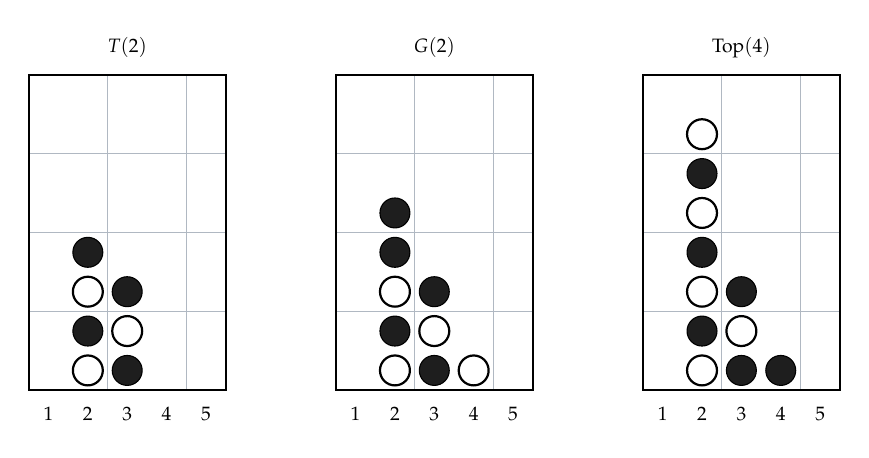
\begin{tikzpicture}[x=0.5cm,y=0.5cm,font=\scriptsize,
  bs/.style={circle,fill=stoneB,draw=black,inner sep=0pt,minimum size=3.8mm},
  ws/.style={circle,fill=white,draw=black,thick,inner sep=0pt,minimum size=3.8mm}]
  \foreach \X/\name/\two/\four in {
      0/{$T(2)$}/{w,b,w,b}/{},
      3.9/{$G(2)$}/{w,b,w,b,b}/{w},
      7.8/{$\Top(4)$}/{w,b,w,b,w,b,w}/{b}} {
    \begin{scope}[xshift=\X cm]
      \draw[gridgray] (0,0) grid (5,8);
      \draw[thick] (0,8) -- (0,0) -- (5,0) -- (5,8) -- cycle;
      \foreach \c in {1,...,5} \node at (\c-0.5,-0.6) {\c};
      \foreach \p [count=\r] in \two {\node[\p s] at (1.5,\r-0.5) {};}
      \node[bs] at (2.5,0.5) {}; \node[ws] at (2.5,1.5) {}; \node[bs] at (2.5,2.5) {};
      \foreach \p [count=\r] in \four {\node[\p s] at (3.5,\r-0.5) {};}
      \node[anchor=south] at (2.5,8.2) {\name};
    \end{scope}}
\end{tikzpicture}
\caption{高度为 $8$（$m=4$）的棋盘上的主线局面，均轮到 $\W$：主干局面 $T(2)$、突围局面 $G(2)=T(2)\cdot\W_4\B_2$，以及墙顶局面 $\Top(4)=T(3)\cdot\W_2\B_4$。}
\label{fig:spine}
\end{figure}

\subsection{每个局面如何闭合}
\label{sec:coverage}

\cref{tab:spine} 中的每个局面，以及 $T(0)$ 处的每个首次应着，都由以下四种方法之一闭合：真实棋盘上的有限证书（“树”）、分区证书（\cref{thm:zones}）、拉伸证书（\cref{thm:stretch}）或拉伸上的分区证书（\cref{thm:sz}）。\cref{tab:coverage} 给出完整的分配，\cref{fig:gwedge} 展示双参数局面族 $G(b)$。

\begin{table}[!htbp]
\centering
\caption{高度 $H=2m$ 的棋盘上各局面的闭合方式。树是针对单一高度的有限证书；\code{Z}$K$ 表示分区高度为 $K$ 的分区证书，对每个偶数 $H\ge K+2$ 有效；\code{S} 表示拉伸。$m\le 4$ 时，$P_{311}$、$P_{322}$ 与 $T(0)$ 的树覆盖了其下的全部局面。}
\label{tab:coverage}
\footnotesize
\begin{tabularx}{\linewidth}{@{}l l l l Y@{}}
\toprule
\textbf{局面} & $m\le 4$ & $m=5$ & $m=6$ & $m\ge 7$ \\
\midrule
空盘，$m=1$ & 树 \code{H2} & & & \\
$P_{311}$ & 树 \code{H4}--\code{H8} & 树 \code{H10} & \code{Z10_311} & \code{Z10_311} \\
$P_{322}$ & 树 \code{H4}--\code{H8} & \code{Z8_322} & \code{Z8_322} & \code{Z8_322} \\
$T(0)$ & 树 \code{H4}--\code{H8} & 主线 & 主线 & 主线 \\
$T(0)\cdot\W_1\B_1$ & & \code{Z8_33311} & \code{Z8_33311} & \code{Z8_33311} \\
$T(0)\cdot\W_3\B_2$ & & 树 \code{H10_U} & \code{Z10_U} & \code{Z10_U} \\
$\Side(b,q)$，$b\in\{1,2\}$，$q\in\{1,5\}$ & & \code{Z8_side}$bq$ & \code{Z8_side}$bq$ & \code{Z8_side}$bq$ \\
$T(1)\cdot\W_3\B_2$，\ $T(2)\cdot\W_3\B_5$ & & \code{Z8_s113}，\code{Z8_s123} & 同左 & 同左 \\
$\Side(b,q)$，$b\ge 3$ & & 认领第~$4$~列 & 同左 & 同左 \\
$\Top(m)$ & & 树 \code{H10_Top} & 树 \code{H12_Top} & \code{STop}：$\Top(5)$ 的拉伸 \\
$G(b)$ & & \multicolumn{3}{l}{见 \cref{fig:gwedge}} \\
\bottomrule
\end{tabularx}
\end{table}

\paragraph{$b\ge 3$ 时的侧着。}在 $\Side(b,q)$（$b\ge 3$）之后，$\B$ 认领第~$4$~列；该列有一颗子，余量为奇数 $2m-1$。后手的所有例外子与潜在例外格都在底部五行内，所以 \cref{thm:claims} 的条件只涉及底部八行。在这八行里，$b\ge 4$ 时墙的样子都相同，所以 $b=3$ 与 $b=4$ 两次有限检查就解决了每个 $b\ge 3$ 与每个偶数高度 $H\ge 2b+2$。这里不需要策略证书 \leanref{C4W5.wall_family_safe}。

\paragraph{拉伸。}有四个证书族用到 \cref{lem:stretchA} 与 \cref{lem:stretchB}，都取 $D=2$：
\begin{itemize}
  \item \code{STop}：高度 $2m$ 上的 $\Top(m)$ 是高度 $10$ 上 $\Top(5)$ 的拉伸，墙在层位 $6$ 处被拉伸 $m-5$~次 \leanref{C4W5.seq_Top}。构建中它用于 $m\ge 7$。
  \item \code{SG3}：高度 $14+2k$ 上的 $G(3)$ 是高度 $14$ 上 $G(3)$ 的拉伸，拉伸发生在所有列之上的层位，只抬高天花板 \leanref{C4W5.seq_G3}。
  \item \code{SG5}：对 $b\ge 5$，高度 $2b+2$ 或 $2b+4$ 上的 $G(b)$（墙顶距天花板一行或三行）是高度 $12$ 或 $14$ 上 $G(5)$ 的拉伸 \leanref{C4W5.seq_G_wall}。
  \item \code{SGZ5R}：对 $b\ge 5$ 与 $m\ge b+3$，$G(b)$ 的底部 $2b+4$~行是 $G(5)$ 底部 $14$~行的拉伸。因此一份以 $G(5)$ 为根、分区高度为 $14$ 的拉伸上的分区证书，覆盖分区高度 $K=2b+4$ 以及每个高度 $2m\ge K+2$（\cref{thm:sz}）。其紧凑数据表对应宽间隙端点 \code{C4W5.SGZLongPacked.g5_wide}，全部分片与端点均已通过 Lean 内核验收。
\end{itemize}

\begin{figure}[!htbp]
\centering
\begin{tikzpicture}[x=0.78cm,y=0.62cm,font=\scriptsize]
  \tikzset{cell/.style={draw=white,thick}}
  \def\cellat#1#2#3#4{\fill[#3,cell] (#1-0.48,#2-0.46) rectangle (#1+0.48,#2+0.46); \node at (#1,#2) {#4};}
  % axes
  \foreach \b in {1,...,8} \node at (\b,1.2) {\b};
  \node at (4.5,0.55) {$b$};
  \foreach \m in {2,...,9} \node[anchor=east] at (0.4,\m) {\m};
  \node[anchor=east] at (-0.2,5.5) {$m$};
  \foreach \m in {2,3,4} {\pgfmathtruncatemacro\top{\m-1}
    \foreach \b in {1,...,\top} {\cellat{\b}{\m}{black!12}{}}}
  \cellat{1}{5}{accent!30}{Z8}
  \foreach \b in {2,3,4} {\cellat{\b}{5}{primary!14}{树}}
  \cellat{1}{6}{accent!30}{Z8} \cellat{2}{6}{accent!30}{Z10}
  \foreach \b in {3,4,5} {\cellat{\b}{6}{primary!14}{树}}
  \foreach \m in {7,8,9} {
    \cellat{1}{\m}{accent!30}{Z8} \cellat{2}{\m}{accent!30}{Z10}
    \cellat{3}{\m}{gold!35}{SG3} \cellat{4}{\m}{accent!30}{Z12}}
  \foreach \b/\m in {5/7,6/7,6/8,7/8,7/9,8/9} {\cellat{\b}{\m}{warn!25}{SG5}}
  \foreach \b/\m in {5/8,5/9,6/9} {\cellat{\b}{\m}{primary!35}{SZ}}
  \begin{scope}[xshift=7.6cm,yshift=1.6cm,x=1cm,y=1cm]
    \foreach \y/\col/\txt in {
      3.6/black!12/{$m\le 4$：包含在 $T(0)$ 的直接树中},
      3.0/primary!14/{真实棋盘上的树（$H=10,12$）},
      2.4/accent!30/{分区证书 \code{Z8_G1}、\code{Z10_G2}、\code{Z12_G4}},
      1.8/gold!35/{\code{SG3}：在所有列之上拉伸},
      1.2/warn!25/{\code{SG5}：拉伸墙，$m\in\{b+1,b+2\}$},
      0.6/primary!35/{\code{SGZ5R}：拉伸上的分区，$m\ge b+3$}} {
      \fill[\col] (0,\y-0.18) rectangle (0.5,\y+0.18);
      \node[anchor=west] at (0.65,\y) {\txt};}
  \end{scope}
\end{tikzpicture}
\caption{高度为 $2m$ 的棋盘上的局面族 $G(b)$，$1\le b\le m-1$。每个格子恰由一份证书闭合。树为 $m=5$ 时的 \code{H10_G2}、\code{H10_G3}、\code{H10_G4} 与 $m=6$ 时的 \code{H12_G3}、\code{H12_G4}、\code{H12_G5}；分区证书为 \code{Z8_G1}（$b=1$，$m\ge 5$）、\code{Z10_G2}（$b=2$，$m\ge 6$）与 \code{Z12_G4}（$b=4$，$m\ge 7$）。}
\label{fig:gwedge}
\end{figure}

\subsection{组装}

对固定高度 $2m$（$m\ge 5$），主线从墙顶向下闭合：先是 $T(m-1)$，其着法 $\W_2$ 通向 $\Top(m)$；然后按 $b$ 递减处理 $T(b)$，其着法 $\W_2$ 通向 $T(b+1)$；最后是 $T(0)$ \leanref{C4W5.T_safe_pos, C4W5.T0_safe}。其余着法都通向 \cref{tab:coverage} 中的局面。加上 $m\le 4$ 的树、开局与镜像对称，就证明了：

\begin{theorem}
\label{thm:even-black}
在每个偶数高度 $h\ge 2$ 上，先手不败。
\lean{C4W5.black_nonloss_five_columns}
\end{theorem}

结合 \cref{prop:white-even}，就得到每个正偶数高度上的和棋 \leanref{C4W5.five_columns_even_draw}。最终紧凑证明使用的三个优化数据表汇总于 \cref{tab:even-certs}。

\begin{table}[!htbp]
\centering
\caption{最终偶数高度开发使用的三张优化数据表。策略行与显式终止见证分别计数。}
\label{tab:even-certs}
\footnotesize
\begin{tabularx}{\linewidth}{@{}l Y r r r@{}}
\toprule
\textbf{证书族} & \textbf{通过内核检查的端点声明} & \textbf{策略行} & \textbf{终止见证} & \textbf{分片} \\
\midrule
\code{SG5} & \code{g5_tight}、\code{g5_mid} & 802{,}510 & 220{,}630 & 697 \\
\code{SGZ5R} & \code{g5_wide} & 905{,}511 & 272{,}542 & 787 \\
\code{STop} & \code{top_all} & 197{,}869 & 37{,}785 & 172 \\
\midrule
\textbf{合计} & \textbf{4 个声明} & \textbf{1{,}905{,}890} & \textbf{530{,}957} & \textbf{1{,}656} \\
\bottomrule
\end{tabularx}
\end{table}

三张表合计包含 $2{,}436{,}847$ 条策略记录与显式终止见证。全部 $1{,}656$ 个分片、三个主声明及四个端点声明均已通过 Lean 内核验收。图 4 中的 SG3 是此前已验收、在紧凑开发中另行暂存的拉伸证书包；本表的 $1{,}656$ 个分片不包含 SG3。最终依赖审计把偶数高度定理追溯到 \code{C4W5.Compact.stretch_families}，再到 \code{C4W5.SG5LongPacked.g5_tight}、\code{g5_mid}、\code{C4W5.SGZLongPacked.g5_wide} 与 \code{C4W5.STopLongPacked.top_all}。早期的 $37$ 族实现（$12{,}554$ 个模块、$1{,}949.40$~MB 生成 Lean 源码）仍作为可复现基线保留；最终统一证明使用的是本表中的紧凑证书族。

% ===== sec7_formal.tex =====
\section{形式化}
\label{sec:formal}

\subsection{三个开发与最终组合}
\label{sec:dev}

Lean 开发包含三个数学部分，均使用工具链 \code{leanprover/lean4:v4.34.0-rc2}。
\begin{itemize}
  \item \emph{无顶条带}：自足文件 \code{FiveColumnsInfinite_PureCore.lean}，只使用 Lean 核心库，不含证书。
  \item \emph{偶数高度}：紧凑版沿用公开定理与 \cref{sec:tools} 中的归约。最终组装保留了此前已验收的 \code{SG3} 包，并使用三个优化数据表 \code{SG5}、\code{SGZ5R} 与 \code{STop}；其端点列于 \cref{tab:even-certs}。
  \item \emph{奇数高度}：该部分加入颜色多态归约（\code{C4W5Gen}）、按位认领检查器、$18$~个证书包以及组装模块 \code{C4W5.Odd.Main}。它与偶数开发共享的 $13$~个 Lean 文件及三个构建配置文件逐字节相同；奇数包只增加自身文件。
\end{itemize}
最终文件 \code{C4W5/FiveColumnsUnified.lean} 引入 \code{C4W5.Even} 与 \code{C4W5.Odd.Main}，通过把 \code{C4W5Gen.five_columns_draw_of_even} 作用于 \code{C4W5.five_columns_even_draw} 得到 \cref{thm:main-finite}。证明依赖审计确认：偶数高度定理实际使用了 \code{SG5} 的两个端点、\code{SGZ5R.g5_wide} 与 \code{STop.top_all}；它们是证明项的依赖，而不只是被导入的模块。

\subsection{公开定理}
\label{sec:public}

\cref{tab:public} 列出公开定理。陈述与 Lean 中一致（\code{open Connect4.NarrowBoards}）。

\begin{table}[!htbp]
\centering
\caption{公开定理。前两条由已经通过内核验收的统一入口 \code{C4W5/FiveColumnsUnified.lean} 证明。}
\label{tab:public}
\small
\begin{tabularx}{\linewidth}{@{}l Y@{}}
\toprule
\textbf{声明} & \textbf{陈述} \\
\midrule
\code{C4W5.five_columns_draw} & \lst{forall h : Nat, IsDraw h (emptyBoard 5)} \\
\code{C4W5.five_columns_neither_player_wins} & 对每个 \lst{h}，任何一方都没有 \lst{exists k, WinFor h p k (emptyBoard 5)} \\
\code{C4W5.five_columns_even_draw} & \lst{forall \{h\}, 2 <= h -> h \% 2 = 0 -> IsDraw h (emptyBoard 5)} \\
\code{C4W5Gen.five_columns_odd_draw} & \lst{forall \{h\}, 1 <= h -> h \% 2 = 1 -> IsDraw h (emptyBoard 5)} \\
\code{C4W5Gen.five_columns_zero_draw} & \lst{IsDraw 0 (emptyBoard 5)} \\
\code{C4W5Gen.five_columns_draw_of_even} & 偶数陈述蕴含 \lst{forall h, IsDraw h (emptyBoard 5)} \\
\code{FiveColumns.five_even_draw_by_stretch} & \lst{FiveColumns.FiveEvenDrawGoal}（\cref{sec:frozen}） \\
\code{FiveColumns.draw_after_center} & \lst{forall \{m\}, 1 <= m -> IsDraw (2*m) (play (emptyBoard 5) 2 .black)} \\
\code{FiveColumns.nonloss_same_column_reply} & 对 \lst{2 <= m} 与每一列 \lst{c}：中央开局、$\W$ 下在 \lst{c} 之后，$\B$ 在 \lst{c} 的应着合法且满足 \lst{C4W5.Safe}，即 \lst{CanAvoidLoss (2*m) .black} \\
\code{C4W5Inf.five_columns_inf_draw} & \lst{IsDrawInf emptyBoard5} \\
\bottomrule
\end{tabularx}
\end{table}

Lean 中列号从 $0$ 开始，所以 \code{play (emptyBoard 5) 2 .black} 就是中央开局。文件 \code{PublicTypeAudit.lean} 用 \code{example} 重新写出偶数定理与两个推论的类型，任何一个类型发生变化都会使构建失败。

\subsection{需要信任什么}
\label{sec:tcb}

定理的可靠程度取决于它们所提到的定义。其余一切，包括每一份证书，都由内核检查。
\begin{itemize}
  \item 上述工具链的 Lean~4 内核，以及公理 \code{propext}、\code{Classical.choice} 与 \code{Quot.sound}。无顶条带定理只用 \code{propext} 与 \code{Quot.sound}。没有证明使用 \code{sorry} 或 \code{native_decide}，也没有声明任何公理。
  \item 下表所列的定义，共 $132$~行。有限高度的定义只用到 Mathlib 中 \code{totalStones} 里对 \code{Fin 5} 的求和与 \code{play} 里的 \code{Function.update}；有限高度部分引入八个基础 Mathlib 模块。
\end{itemize}
\begin{center}
\small
\begin{tabularx}{\linewidth}{@{}l l Y@{}}
\toprule
\textbf{文件} & \textbf{行} & \textbf{定义} \\
\midrule
\code{experiments/NarrowBoards.lean} & 47--65 & \code{Board}、\code{emptyBoard}、\code{Legal}、\code{Valid}、\code{BoardFull}、\code{play}、\code{stone} \\
 & 96--112 & \code{cellAtInt}、\code{HasFourDir}、\code{HasFour} \\
 & 290--292 & \code{totalStones}、\code{toMove} \\
 & 351--366 & \code{SafeFor}、\code{CanAvoidLoss}、\code{IsDraw} \\
 & 376--385 & \code{WinFor}（仅 \code{five_columns_neither_player_wins} 用到） \\
\code{Connect4Proof/Basic.lean} & 14--23 & \code{Player}、\code{opponent} \\
\code{FiveColumnsInfinite_PureCore.lean} & 18--74 & 条带版本自带的一份上述定义，以及 \code{SafeForInf}、\code{CanAvoidLossInf}、\code{IsDrawInf} \\
\bottomrule
\end{tabularx}
\end{center}
搜索策略、写出证书的 C++ 与 Python 程序不需要信任。错误的应着、缺失的分支或格式错误的键都会使内核检查求值为 \code{false}，构建随之失败。

\subsection{规则的第二份副本}
\label{sec:frozen}

偶数高度定理还针对规则的第二份副本陈述。\code{FiveColumns.FiveEvenDrawGoal} 是用 \code{Connect4.FourColumns} 的定义写成的陈述 \lst{forall m, 1 <= m -> IsDraw (2*m) (emptyBoard 5)}；\code{Connect4.FourColumns} 是为窄棋盘工作编写并冻结的另一个文件 \cite{narrow14,fourcol}。定理 \code{FiveColumns.draw_iff_narrowBoards} 证明两份副本对每个宽度、高度与局面定义出相同的 \code{IsDraw}。这防止了在五列项目进行中规则被意外改动。

\subsection{证书如何被检查}

证书是一张有限的表，存为自然数的平衡二叉搜索树，把编码后的局面映射到应着（\cref{sec:odd-black} 的控制器证书只列出局面）。每类证书都有一个检查器，即一个 Lean 函数，只有当每个存储的局面都通过 \cref{sec:tools} 中相应定理的封闭条件时才返回 \code{true}；还有一个可靠性定理，说明 \code{true} 蕴含不败。内核用 \code{decide +kernel} 在证书上对检查器求值。大证书被切成分块分别检查，再合并。\cref{app:kernel} 介绍编码方式，以及使内核求值足够快的技术。

\subsection{构建记录与独立核验}
\label{sec:receipts}


\begin{table}[!htbp]
\centering
\caption{最终 Lean 构建回执，工具链为 \code{leanprover/lean4:v4.34.0-rc2}。}
\label{tab:receipts}
\footnotesize
\begin{tabularx}{\linewidth}{@{}L{2.35cm} L{4.15cm} Y L{2.6cm}@{}}
\toprule
\textbf{开发} & \textbf{目标} & \textbf{结果} & \textbf{公理} \\
\midrule
无顶条带 & \code{FiveColumnsInfinite_PureCore.lean} & 单独构建，2.4\,秒 & \code{propext}、\code{Quot.sound} \\
奇数高度，$h=0$ & \code{C4W5.Odd.Main} & 1{,}117 个任务全部通过 & 三条标准公理 \\
紧凑偶数高度 & \code{SG5}、\code{SGZ5R}、\code{STop} & 1{,}656 个分片；三个主声明与四个端点全部通过内核验收 & 三条标准公理 \\
统一有限高度 & \code{C4W5.FiveColumnsUnified} & 1{,}014 个依赖模块：894 个新构建、120 个经核验复用；最终端点通过 & 三条标准公理 \\
\bottomrule
\end{tabularx}
\end{table}

最终组装直接合并了三张优化表的对象，没有重新编译或重新计算表数据。此前已验收的 \code{SG3} 包另行暂存；\cref{tab:even-certs} 中的 $1{,}656$ 个分片仅指这三张优化表。新的 Lean 进程重新检查了公开端点类型，并对 \code{C4W5.five_columns_even_draw}、\code{C4W5.five_columns_draw} 与 \code{C4W5.five_columns_neither_player_wins} 打印公理；三者恰好都只依赖 \code{propext}、\code{Classical.choice} 与 \code{Quot.sound}。证明依赖审计把偶数高度定理追溯到 \code{C4W5.Compact.stretch_families}，再到 \code{g5_tight}、\code{g5_mid}、\code{g5_wide} 与 \code{top_all}。最终统一依赖图共有 $1{,}014$ 个模块，其中 $894$ 个在最终组装中构建，另有 $120$ 个在源码沿袭与产物哈希核验后复用。

与最终构建相互独立的核验：
\begin{itemize}
  \item 全部 $18$~个奇数高度证书包都由独立 C++ 程序逐位重新生成，SHA-256 摘要一致；
  \item 三张紧凑表的源码清单与远端读回哈希一致，各自的验收记录均显示全部分片、主声明与端点通过 Lean 内核；
  \item 项目源码审计未发现 \code{sorry}、\code{admit}、\code{axiom}、\code{native_decide}、\code{ofReduceBool}、\code{trustCompiler} 或 \code{extern}；
  \item 一个从零编写、与项目不共享任何代码的独立求解器，复现了 \cref{sec:odd} 与 \cref{sec:even-black} 中引用的每一个博弈值（\cref{app:recheck}）。
\end{itemize}

\paragraph{认领叶与紧凑证书。}紧凑证明原样沿用定义与公开陈述，但用带认领叶的较小证书替换了早期的有限树与分区树（\cref{app:compression}）。高度至多为 $8$ 的有限根由 \code{C4W5.Compact.SmallComplete} 组合；$13$ 个固定分区证书族共有 $361{,}155$ 条存储记录，而原版为 $4{,}226{,}645$ 条。\cref{tab:even-certs} 中的三个长程表族完成拉伸与拉伸上的分区部分。因此，紧凑开发就是最终定理所使用的证明，而不是一套并行实验。

\subsection{来源}

数学内容、搜索程序与 Lean 证明由署名的几个 AI 系统完成，它们在各自独立的会话中工作，由一位人类协调者统筹：协调者在会话之间传递材料，安排本地硬件上的长时间计算，并决定项目方向。最终紧凑表对象直接并入统一开发，没有重新计算表数据；所得公开定理由 Lean 内核检查。随本文发布的仓库记录了这一工作流程，包括窄棋盘上的配套工作 \cite{narrow14,fourcol} 与形式化存档 \cite{c4w5archive}。

% ===== sec8_open.tex =====
\section{开放问题}
\label{sec:open}

\begin{enumerate}
  \item \emph{六列。}Tromp 的表给出：$6\times4$、$6\times6$、$6\times8$ 后手胜，$6\times5$ 和棋，$6\times7$、$6\times9$ 先手胜 \cite{tromp2026}。博弈值随高度变化，所以关于六列的一般定理必须证明取胜，而不只是不败。下移、认领与分区都是为不败而陈述的；拉伸与分区能否为强制取胜提供证书，尚不清楚。
  \item \emph{拉伸是否必要？}\cref{sec:counterexamples} 的反例迫使在所有高度上使用同一开局的策略走上主线 $333$，而沿这条主线 $\W$ 可以筑起任意高度的墙。我们不知道依赖于高度的策略、或不同的不变量，能否避开无界的墙，从而避开拉伸。
  \item \emph{偶数高度先手的可读策略。}其余五种情形的策略都能写在一页之内。偶数高度先手的证明仍有相当一部分由证书承担。哪怕是一份未经形式化的简短描述，也会是真正的进步。
  \item \emph{进一步压缩。}当前紧凑证明用 $1{,}656$ 个分片闭合三个长程证书族。能否在保持覆盖范围的同时，进一步减少存储的策略行，或给出更直接的数学描述，仍值得研究。
  \item \emph{条带上策略的形式化。}\cref{lem:koenig} 只在纸面上证明。把它形式化，就能把 \cref{thm:main-inf} 变成关于无限对局策略的陈述。
\end{enumerate}

% ===== refs.tex =====
\begin{thebibliography}{12}
\small\raggedright
\setlength{\itemsep}{3pt}

\bibitem{allis1988}
{\latinrm
L.~V. Allis.
\newblock \emph{A Knowledge-Based Approach of Connect-Four. The Game is Solved: White Wins}.
\newblock Master's thesis, Vrije Universiteit Amsterdam, Report IR-163, October 1988.
\newblock \url{https://tromp.github.io/c4/connect4_thesis.pdf}.}

\bibitem{allen1989}
{\latinrm J.~D. Allen.
\newblock A note on the computer solution of Connect-Four.
\newblock In D.~N.~L. Levy and D.~F. Beal (eds.), \emph{Heuristic Programming in Artificial Intelligence: The First Computer Olympiad}, pages 134--135. Ellis Horwood, 1989.}

\bibitem{tromp2026}
{\latinrm J.~Tromp.
\newblock \emph{John's Connect Four Playground}.}
\newblock \url{https://tromp.github.io/c4/c4.html}，访问于 2026 年 11 月。

\bibitem{steininger2026}
{\latinrm C.~Steininger.
\newblock \emph{A fast Connect 4 solver}.}
\newblock GitHub 仓库及结果表，\url{https://github.com/ChristopheSteininger/c4}，访问于 2026 年 11 月。

\bibitem{yamaguchi2012}
{\latinrm
Y.~Yamaguchi, K.~Yamaguchi, T.~Tanaka, and T.~Kaneko.
\newblock Infinite Connect-Four is solved: Draw.
\newblock In \emph{Advances in Computer Games (ACG 2011)}, LNCS 7168, pages 208--219. Springer, 2012.
\newblock \href{https://doi.org/10.1007/978-3-642-31866-5_18}{doi:10.1007/978-3-642-31866-5\_18}.}

\bibitem{yamaguchi2014}
{\latinrm
Y.~Yamaguchi, T.~Tanaka, and K.~Yamaguchi.
\newblock Cylinder-Infinite-Connect-Four Except for Widths 2, 6, and 11 Is Solved: Draw.
\newblock In A.~Plaat, H.~J. van den Herik and W.~A. Kosters (eds.), \emph{Computers and Games}, LNCS 8427, pages 163--174. Springer, 2014.
\newblock \href{https://doi.org/10.1007/978-3-319-09165-5_14}{doi:10.1007/978-3-319-09165-5\_14}.}

\bibitem{lean4}
{\latinrm
L.~de~Moura and S.~Ullrich.
\newblock The Lean 4 theorem prover and programming language.
\newblock In \emph{Automated Deduction -- CADE 28}, LNCS 12699, pages 625--635. Springer, 2021.
\newblock \href{https://doi.org/10.1007/978-3-030-79876-5_37}{doi:10.1007/978-3-030-79876-5\_37}.}

\bibitem{mathlib}
{\latinrm
The mathlib Community.
\newblock The Lean mathematical library.
\newblock In \emph{Proceedings of the 9th ACM SIGPLAN International Conference on Certified Programs and Proofs (CPP 2020)}, pages 367--381. ACM, 2020.
\newblock \href{https://doi.org/10.1145/3372885.3373824}{doi:10.1145/3372885.3373824}.}

\bibitem{narrow14}
{\latinrm GPT and Claude.}
\newblock 一至四列重力四子棋的和棋策略：覆盖策略、最优主动换列次数与 Lean 验证。研究手稿，2026。\url{https://github.com/wugang6812/narrow-connect-four/blob/v0.3.0/papers/paper-zh.pdf}。

\bibitem{fourcol}
{\latinrm GPT and Claude.}
\newblock 四列重力四子棋的统一回应算法与交替段压缩。研究手稿，2026。\url{https://github.com/wugang6812/narrow-connect-four/blob/v0.3.0/papers/algorithm-zh.pdf}。

\bibitem{c4w5archive}
五列四子棋全高度证明的 Lean~4 源码、证书与内核验收日志。\url{https://github.com/wugang6812/five-column-connect-four/releases/tag/v1.0.0}。

\end{thebibliography}

% ===== app.tex =====
\appendix

\section{让内核完成检查}
\label{app:kernel}

每份证书都通过内核归约检查（\code{decide +kernel}），从不借助编译代码（\code{native_decide}）。内核惰性地归约项，并且只对自然数字面量有快速算术，所以检查器的写法是让所有数据都保持为字面量，并尽早强制求值。

\begin{itemize}
  \item \emph{局面。}一个局面是十个自然数：每列一个先手子的位掩码和该列的高度。后手子的掩码是 $(2^{h_c}-1)\oplus b_c$。四连由移位掩码的十一个按位合取检测，一个引理证明这一检测与 $\HasFour$ 一致 \leanref{hasFourF_iff}。
  \item \emph{强制求值。}一个续延传递风格的辅助函数 \code{force n f} 在 \code{f} 运行之前先对字面量 \code{n} 做模式匹配，使内核用字面量算术求出它，而不是展开定义。
  \item \emph{查找。}内核访问数组元素的时间与下标成线性关系，所以证书是字面量的平衡二叉搜索树。局面及其应着被打包成一个键，只使用奇数基数（认领与分区的键用 $513$、$11$、$243$ 与 $3125$；拉伸的键用 $2^{89}-1$、$131$ 与 $5^{10}$）。区间查询 \code{raw lo hi t} 寻找满足 $\mathrm{lo}\le w<\mathrm{hi}$ 的键 $w$，每个节点只做两次比较、不做除法。带标签的查找取 $\mathrm{hi}=\mathrm{lo}+3125$，应着位于最低一位；控制器证书的点查找取 $\mathrm{hi}=\mathrm{lo}+1$。可靠性来自打包在有界数位上的单射性 \leanref{unpack9_key9, decodeZ9}，无需证明树是有序的。
  \item \emph{认领。}经过一个格子的十二条非竖直线，由在掩码上对四列窗口的六次扫描来检查 \leanref{checkLinesG}；同一段代码服务于两种奇偶情形 \leanref{fastOdd_sound, fastEven_sound}。
  \item \emph{拉伸。}为了按拉伸意义判定成员资格，检查器提出一个未拉伸的局面，并通过再次正向拉伸来验证它 \leanref{normAt, stretchPos}，所以寻找原像的过程不必被信任。
  \item \emph{模块。}大证书被切成至多含 $512$~个局面的分块。分块放在数据模块中（作为声明为 \code{noncomputable} 的子树，不为其生成编译代码，内核归约不受影响）；每个分块在检查模块中由各自的内核定理检查，合并定理再沿搜索树顶部把结果组合起来。检查模块可以逐个构建，以限制内存。
\end{itemize}

\section{有限树中的认领叶}
\label{app:compression}

本附录解释最终紧凑证明所使用的认领叶压缩。偶数高度先手的原始有限树生成于奇数高度的按位认领检查器出现之前，它们把每条分支一直展开到四连或满盘。偶数高度上轮到 $\W$ 时 $\eps=1$，与奇数高度后手的情形相同，所以奇数高度的认领检查器可以原样使用：一着应着若通向满足 \cref{thm:claims} 的局面，树就可以在那里结束，且不占存储。重新选择应着、尽早到达这类叶，就得到 \cref{tab:compression} 中的替换证书；每份都作为对所替换之树同一陈述的证明，经过内核检查。

\begin{table}[!htbp]
\centering
\caption{带认领叶的替换证书。计数为每个根存储的策略条目；认领叶不占存储，单独计数。}
\label{tab:compression}
\footnotesize
\begin{tabularx}{\linewidth}{@{}l l r r r Y@{}}
\toprule
\textbf{高度，根} & \textbf{Lean 命名空间} & \textbf{之前} & \textbf{之后} & \textbf{变化} & \textbf{认领叶，内核时间} \\
\midrule
$H=6$：$311$、$322$、$333$ & \code{EvenClaimPilot} & 58{,}978 & 6{,}455 & $-89.06\%$ & 5{,}351 个叶；98.3\,秒 \\
$H=8$：$311$ & \code{EvenClaimSharded.H8_311} & 114{,}402 & 12{,}774 & $-88.83\%$ & 8{,}338 个叶；26 片，221.0\,秒 \\
$H=8$：$322$ & \code{H8_322_known_dag} & 87{,}021 & 593 & $-99.32\%$ & 1{,}449 个叶；15.9\,秒 \\
$H=8$：$333$ & \code{EvenClaimSharded.H8_333} & 417{,}473 & 45{,}606 & $-89.08\%$ & 22{,}919 个叶；98 片，776.3\,秒 \\
$H=8$，合计 & & 618{,}896 & 58{,}973 & $-90.47\%$ & 125 个模块 \\
$H=10$：$\Top(5)$ & \code{WideRealPilot.H10_Top} & 7{,}861 & 1{,}390 & $-82.32\%$ & 408 个叶；18.4\,秒 \\
\bottomrule
\end{tabularx}
\end{table}

这些百分比只针对这些有限根，不适用于整个偶数高度证明；长程部分由 \cref{tab:even-certs} 中的紧凑表族闭合。对高度 $10$ 上的 $\Top(5)$，原树的编码超出了奇数检查器的键范围；一个适配器证明原来的宽键可以用同一认领测试检查 \leanref{safeP_of_wide_claimOdd_tree}。最终紧凑构建使用高度至多为 $8$ 的紧凑有限证书；在高度 $2$ 到 $8$ 上，它们存储 $65{,}563$~条策略条目而非 $679{,}874$~条，Lean 源码为 $2.7$~MB 而非 $46.3$~MB。

\section{对所引博弈值的独立复算}
\label{app:recheck}

\cref{sec:odd} 与 \cref{sec:even-black} 中引用的博弈值不属于形式证明，它们只解释证明的形状。这些值由一个独立于项目编写的求解器复算（带置换表的位棋盘与或搜索，对双方分别判定能否强制连成四子；它曾在 $5\times 4$ 棋盘上，对长度为一至四步的全部 $780$~个着法序列之后的局面，与朴素极小极大搜索交叉核对）。结果见 \cref{tab:recheck}。着法串列出所下各列，第一着属于 $\B$；值是双方都最优时所得局面的结果。

\begin{table}[!htbp]
\centering
\caption{独立求解器复算的值。对主线上轮到 $\W$ 的局面，“$\B$ 胜”表示 $\B$ 的应着绰绰有余。}
\label{tab:recheck}
\footnotesize
\begin{tabularx}{\linewidth}{@{}l l l Y@{}}
\toprule
\textbf{棋盘} & \textbf{着法} & \textbf{值} & \textbf{用于} \\
\midrule
$5\times4$ & $1$；\ $5$ & $\W$ 胜；\ $\W$ 胜 & 边列开局会输（\cref{sec:counterexamples}） \\
$5\times8$ & $22$ & $\W$ 胜 & $\B_2$ 会输 \\
$5\times8$ & $331$、$332$、$334$、$335$ & 均为 $\W$ 胜 & $\B_3\W_3$ 之后只有跟盖能和 \\
$5\times8$ & $333$ & 和 & \\
\midrule
$5\times5$ & $2$ & 和 & 首着第~$2$~列 \\
$5\times7$ & $2$ & 和 & \\
$5\times5$ & $23$；\ $22$ & $\B$ 胜；\ 和 & 高度 $5$ 的切换（\cref{sec:odd-white}） \\
$5\times7$ & $23$；\ $22$ & 和；\ 和 & \\
$5\times9$ & $23$；\ $22$ & 和；\ $\B$ 胜 & 两种应着都不能在所有奇数高度上成立 \\
$5\times5$、$5\times7$、$5\times9$ & $12$；\ $32$ & 和；\ 和 & 对 $\B_1$、$\B_3$ 的应着 \\
\midrule
$5\times10$、$5\times12$ & $333\,(22)^3\,14$ & $\B$ 胜 & $\Side(3,1)$ \\
$5\times10$、$5\times12$ & $333\,(22)^3\,34$ & 和 & $\Side(3,3)$ \\
$5\times10$、$5\times12$ & $333\,(22)^3\,54$ & $\B$ 胜 & $\Side(3,5)$ \\
$5\times10$ & $333\,(22)^4\,24$ & 和 & $\Top(5)$ \\
$5\times12$ & $333\,(22)^5\,24$ & 和 & $\Top(6)$ \\
$5\times10$ & $333\,(22)^4\,22$ & $\W$ 胜 & 在墙顶跟盖会输 \\
$5\times12$ & $333\,(22)^5\,22$ & $\W$ 胜 & \\
$5\times10$ & $333\,22\,42$；\ $333\,(22)^2\,42$ & $\B$ 胜；\ $\B$ 胜 & $G(1)$、$G(2)$ \\
\midrule
$5\times1$ 至 $5\times6$ & 空盘 & 和 & 小高度上的 \cref{thm:main-finite} \\
$6\times4$、$6\times5$、$6\times6$ & 空盘 & 后手胜；和；后手胜 & 与 Tromp 的表一致 \cite{tromp2026} \\
\bottomrule
\end{tabularx}
\end{table}

\clearpage
\section{Lean 声明索引}
\label{app:index}

\cref{tab:index} 对本文的每个结果列出它所在的 Lean 模块，以及陈述或证明它的声明；声明名省略了命名空间。

\begin{table}[!htbp]
\centering
\caption{本文的结果及陈述它们的 Lean 声明。除标注“顶层”者外，模块路径相对于 \code{C4W5/}。}
\label{tab:index}
\scriptsize
\renewcommand{\arraystretch}{1.25}
\begin{tabularx}{\linewidth}{@{}L{3.3cm} L{3.9cm} Y@{}}
\toprule
\textbf{结果} & \textbf{模块} & \textbf{声明} \\
\midrule
规则、不败、和棋（\cref{sec:rules}） & \code{experiments/NarrowBoards}（顶层） & \code{Board}，\code{play}，\code{HasFour}，\code{SafeFor}，\code{CanAvoidLoss}，\code{IsDraw}，\code{WinFor}，\code{draw_excludes_forced_wins} \\
无顶条带（\cref{prop:inf-black}、\cref{prop:white-even}、\cref{thm:main-inf}） & \code{FiveColumnsInfinite_PureCore}（顶层） & \code{SafeForInf}，\code{IsDrawInf}，\code{BInfInv}，\code{black_nonloss_inf}，\code{WInfInv}，\code{white_nonloss_inf}，\code{five_columns_inf_draw} \\
偶数高度后手（\cref{prop:white-even}） & \code{Allis/Columns}，\code{Allis/Geometry}，\code{Allis/Strategy} & \code{SOdd}，\code{SEven}，\code{SQ}，\code{SOpen}，\code{WD}，\code{W2}，\code{W3}，\code{white_nonloss_five} \\
下移、认领（\cref{lem:shiftdown}、\cref{thm:claims}） & \code{Theory/ShiftDownGen}，\code{Theory/ClaimGen} & \code{ExceptionalP}，\code{PotExcP}，\code{exists_exceptional_in_line_gen}，\code{CInvGen}，\code{ClaimOddHyp}，\code{ClaimEvenHyp}，\code{claim_odd_safe}，\code{claim_even_safe} \\
分区（\cref{thm:zones}） & \code{Theory/ZoneGen}，\code{Theory/ClaimLeafBridge} & \code{truncG}，\code{LabG}，\code{DiscEP}，\code{TColP}，\code{ZoneCert2P}，\code{oppFour_low}，\code{zone_safeL_gen}，\code{claimOdd_zoneLeafSound}，\code{claimEven_zoneLeafSound} \\
以 $\B$ 为防守方的版本 & \code{Theory/ShiftDown}，\code{Theory/Claim}，\code{Theory/Zone}，\code{Theory/ZoneL} & \code{exists_exceptional_in_line}，\code{claim_safe}，\code{zone_safeL} \\
拉伸（\cref{lem:stretchA}、\cref{lem:stretchB}、\cref{thm:stretch}、\cref{thm:sz}） & \code{Theory/Stretch}，\code{Theory/StretchB}，\code{Theory/StretchGame}，\code{Theory/StretchZone} & \code{Landmark}，\code{ClearCut}，\code{stretch}，\code{hasFour_stretch_iff}，\code{SEq}，\code{SEq.play}，\code{exists_variant}，\code{stretch_safe}，\code{stretch_safeL}，\code{SZCert}，\code{zoneCert2_of_sz}，\code{sz_safe} \\
检查器与键（\cref{app:kernel}） & \code{Odd/FastKey}，\code{Odd/ClaimBitsGen}，\code{Odd/RealGen}，\code{Odd/ZoneFastGen} & \code{key9}，\code{raw_sound}，\code{fastOdd_sound}，\code{fastEven_sound}，\code{safeP_of_real_tree}，\code{zone_safeP_of_tree} \\
奇数高度先手（\cref{thm:odd-black}） & \code{Odd/OddBlackController}，\code{Odd/OddBlackExplicit} & \code{oddBlackCap4Line}，\code{oddBlackRealReply}，\code{oddBlackZoneCapReply}，\code{odd_black_nonloss} \\
奇数高度后手（\cref{thm:odd-white}） & \code{Odd/OddWhite} & \code{empty_white_safe_of}，\code{b2w3_white_safe_of}，\code{odd_white_nonloss} \\
偶数高度先手（\cref{thm:even-black}） & \code{Compact/*}，\code{SG5LongPacked}，\code{SGZLongPacked}，\code{STopLongPacked} & \code{T_safe_pos}，\code{T0_safe}，\code{wall_family_safe}，\code{stretch_families}，\code{g5_tight}，\code{g5_mid}，\code{g5_wide}，\code{top_all}，\code{five_columns_even_draw} \\
开局（\cref{cor:centre}）、规则的第二份副本（\cref{sec:frozen}） & \code{FiveColumns/OptimalOpening}，\code{FiveColumns/FrozenBridge}（顶层） & \code{draw_after_center}，\code{nonloss_same_column_reply}，\code{draw_iff_narrowBoards}，\code{five_even_draw_by_stretch} \\
所有高度（\cref{thm:main-finite}） & \code{Odd/Main}，\code{FiveColumnsUnified} & \code{five_columns_zero_draw}，\code{five_columns_odd_draw}，\code{five_columns_draw_of_even}，\code{five_columns_draw}，\code{five_columns_neither_player_wins} \\
\bottomrule
\end{tabularx}
\end{table}

\end{document}
